\documentclass[12pt,onecolumn]{report}


\usepackage[table,xcdraw]{xcolor}
\usepackage{array}
\usepackage{ulem}
\usepackage{amsmath}
\usepackage{algorithm}
\usepackage{algpseudocode}
\sloppy
\renewcommand{\thesection}{\thechapter.\arabic{section}}
\renewcommand{\thesubsection}{\thesection.\arabic{subsection}}
\renewcommand{\thesubsubsection}{\thesubsection.\arabic{subsubsection}}

% -------------------- Document Layout --------------------

\usepackage{geometry}        % For page layout
\geometry{
    a4paper,                 % Paper size
    margin=0.5in,            % General margin
    top=1in,                 % Top margin
    bottom=1in,              % Bottom margin
    left=0.6in,              % Left margin
    right=0.6in              % Right margin
}

% -------------------- Header and Footer Setup --------------------

\usepackage{fancyhdr}        % For custom headers and footers
\usepackage{xcolor}          % For text color customization

\pagestyle{fancy}            % Set fancy header/footer style
\renewcommand{\headrulewidth}{0.4pt}   % Header rule thickness
\renewcommand{\footrulewidth}{0.4pt}   % Footer rule thickness
\setlength{\headheight}{24.65pt} % Header height (adjust as needed)

% Define custom color
\definecolor{lightgray}{gray}{0.7}

% Clear existing header and footer settings
\fancyhf{}

% Set up the left, center, and right parts of the header
\lhead{\textit{\textcolor{lightgray}{\small Jason Joel Pinto}}} % Left header
\chead{}                                                       % Center header (empty)
\rhead{\hfill \textit{\textcolor{lightgray}{\small Uncertainty-Aware Deep Learning for Early Detection of Alzheimer’s Disease Using MRI images Data}}} % Right-aligned header

% Set up the left, center, and right parts of the footer
\lfoot{\textit{\textcolor{lightgray}{\small Gisma University of Applied Sciences}}}  % Left footer
\cfoot{\textcolor{lightgray}{\large \bfseries \thepage}}                             % Center footer (page number)
\rfoot{\hfill \textit{\textcolor{lightgray}{\small December, 2024}}}                % Right footer with date

\renewcommand{\headrulewidth}{0.4pt}
\renewcommand{\footrulewidth}{0.4pt}
\setlength{\headheight}{10pt}
\renewcommand{\headrule}{\textcolor{lightgray}{\rule{\textwidth}{0.3pt}}}
\renewcommand{\footrule}{\textcolor{lightgray}{\rule{\textwidth}{0.3pt}}}

% -------------------- Font and Text Customization --------------------

\usepackage[utf8]{inputenc}  % UTF-8 encoding
\usepackage[T1]{fontenc}     % Font encoding
\usepackage{ebgaramond}      % Use EB Garamond font
% \usepackage{mathptmx}      % Use EB Garamond font
\usepackage{caption}         % For customizing captions

% Set caption style to small and italic
\captionsetup{font={small,it} }  % small font and italic style for captions

% -------------------- Line Spacing --------------------

\usepackage{setspace}        % For line spacing
\onehalfspacing              % Set line spacing to 1.5

% -------------------- Title and Section Formatting --------------------

\usepackage{titlesec}        % For title formatting
\titleformat{\title}[block]
  {\normalfont\bfseries\Huge}{\thetitle}{0pt}{}  % Title formatting (Huge font size, bold)

\titleformat{\chapter}[block]
  {\normalfont\bfseries\LARGE}{}{0pt}{\Large}     % Chapter headings (LARGE font size, bold)
  
\titleformat{\section}
  {\normalfont\Large\bfseries}{\thesection}{1em}{}  % Section headings (Large font size, bold)

\titleformat{\subsection}
  {\normalfont\normalsize\bfseries}{\thesubsection}{1em}{}  % Subsection headings (normal size, bold)

\titlespacing*{\chapter}{0pt}{-10pt}{15pt}   % Adjust chapter spacing

\usepackage{chngcntr}
\counterwithin{chapter}{part}

\titleformat{\chapter}[block]
  {\normalfont\bfseries\LARGE}{Chapter \thechapter}{1em}{\Large}

\titleformat{\chapter}[display]
{\normalfont\bfseries\LARGE}   % Font style and size for the chapter title
{Chapter \thechapter}         % "Chapter X" text
{1em}                         % Spacing between "Chapter X" and the title
{\Large}                      % Font size for the chapter title on a new line

% -------------------- Page Break Management --------------------

% Remove page breaks between chapters
% \newcommand{\chapterbreak}{\vspace{1.5cm}} % Adjust spacing if needed
% \titleclass{\chapter}{straight}[\chapterbreak] 

% -------------------- Bibliography and Citations --------------------

\usepackage[backend=biber]{biblatex}  % For bibliography management
\addbibresource{mybib.bib}            % Add .bib file for references

% -------------------- Hyperlinks --------------------

\usepackage{hyperref}        % For clickable links
\hypersetup{
    colorlinks=true,
    linkcolor=blue,
    urlcolor=blue,
    citecolor=blue
}

% -------------------- Images and Captions --------------------

\usepackage{graphicx}        % For including images
\usepackage{caption}         % For customizing captions
\usepackage{enumitem}        % For customizations like "nosep"


% Begin document
\begin{document}

% Title page
%\begin{titlepage}
%    \centering
%    {\bfseries\Huge Early Prediction and Progression Modelling of Alzheimer’s Disease Using Multi-Modal Time Series Data \par} % Title (22pt, bold)
%    \vspace{1.5cm}
%    {\Large Jason Joel Pinto \par} % Author name (14pt)
%    \vfill
%    A Thesis Submitted in Partial Fulfillment of the Requirements for the Degree of \par
%    {\large MSc in Data Science, AI and Digital Marketing \par} % Program (12pt)
%    \vspace{1cm}
%    {\large Gisma University of Applied Sciences \par} % University (12pt)
%    {\large Dec, 2024 \par} % Month and year (12pt)
%    \vfill
%\end{titlepage}

\begin{titlepage}
    \begin{center}
        % University Logo (Optional)
        % \includegraphics[width=0.15\textwidth]{university_logo.png} \\[1cm]
        
        % University Name
        \textsc{\Large Gisma University of Applied Sciences} \\[1.5cm]
        \vfill  
        % Title
        % \rule{\linewidth}{0.2mm} \\[0.4cm]
        {\bfseries\Huge Uncertainty-Aware Deep Learning for Early Detection of Alzheimer’s Disease Using MRI Images Data \\[0.4cm]}
        % \rule{\linewidth}{0.2mm} \\[1.5cm]
        \vfill        
        % Author Name
        {\Large \textbf{Jason Joel Pinto}} \\[2cm]
        \vfill
        % Submission Text
        {\large A Thesis Submitted in Partial Fulfillment of the Requirements for the Degree of} \\[0.5cm]
        {\Large MSc in Data Science, AI and Digital Marketing} \\[1.5cm]
        
        % Date
        {\large December, 2024}
        
        \vfill
    \end{center}
\end{titlepage}

% Abstract
\chapter*{Abstract}
\addcontentsline{toc}{chapter}{Abstract}

Alzheimer's is a neurological disorder, which is a main cause for dementia \cite{Ewers2011}. There are a lot of researches are that being conducted right now all over the world for the Alzheimer disease. A disease such as alzheimer's is very hard to predict as studies show that it can be cause due to multiple factors. Now when it comes to Multi modal machine learning models, it integrates different data sources such as a persons demographic data, lifestyle, medical history, clinical assessment, and cognitive assessment etc. This has sparked a new idea to process the data and understand a patter to detect the disease at a early stage. To achieve this various advanced machine learning models are being used.

As new advancement are being done in the medical fields, the aged population is going to rise. And more and more people, their relatives and family members are going to face deadly diseases such as Alzheimer's. Studies has shown that the early detection of alzheimer's Disease is more likely to get treated or leads to less serious problems when compared to the medications started at a later stage \cite{Cummings2024}.

For this study the data being used is based on the Alzheimer's research organization called Open Access Series of Imaging Studies (OSIS). Various traditional as well and deep learning models are used to find the best model as well as the best parameters in order to reach a most accuracy score possible. The measurement scores used to select the best model out of all will be Recall, Accuracy, F1-score and Precision. 

Incomplete.... Need to fill the rest.


% Acknowledgments
% \chapter*{Acknowledgments}
% \addcontentsline{toc}{chapter}{Acknowledgments}
% Write your acknowledgments here.

% Table of contents
\tableofcontents
\listoffigures % Optional
\listoftables  % Optional

% Chapters
\chapter{Introductions}

Alzheimer's is a neurological problem that starts with a build up of proteins called amyloid plaques and neurofibrillary tangles. This leads to the brain cells to die over time and this leads to the shrinkage of the brain size\cite{mayo_alzheimers_2024}. Studies show us that about 5.4 million people in the States have Alzheimer's. And the studies show upward trend in the newer generations in getting Alzheimer's Disease. It is expected to increase by 10 million people. As of today every 68 second and new person is being diagnosed by Alzheimer's Disease. And the studies show that by 2050 this is going to decrease to 33 seconds\cite{2012131}. Between the year 2000 and 2017 the deaths reported due to alzheimer's have been increased by 143 \%\cite{2019321}. Alzheimer's is a disease which get's worse over the years, it keeps on progressing and the worst thing it is not reversible. Once worsened a lot of time and efforts go into the alzheimer's diseace. Which might end up being one of the costliest disease for any countries economy\cite{10.3389/fnagi.2024.1363458}. Hence it becomes very important that it is diagnosed as a early stage so that it can be controlled and treated. If it is detected early then doctor's with the help of medications can make sure that brain damage is not worsened. Currently magnetic resonance imaging (MRI),functional magetic resonance imaging(fMRI), computer tomography and positron emission tomography (PET) are used in order to early detect the Alzheimer's disease. These technologies are very expensive, very time consuming task and not very accessible for everyone as it Requirement sophisticated machines.

Machine Learning can be used to find if there is a way where one can find if there is a way models can find patterns which makes it possible to detect the disease at even earlier stage. As there are various studies that are being conducted all around the world, there are various data that are available which can be used by the machine learning models to analyze and early detect the disease. Based on prior researches, the researchers have numerical data's related to a persons MRI's and biomarkers in a persons body. With help of these they find whether a person is demented or not. If these data are used and ML model be developed which will be able to predict the will be lead to inexpensive diagnosis and can be made easily available to more and more people. In addition to that the automated model will be more accurate and also removes all human errors. 

\begin{figure}[h!]
    \centering
    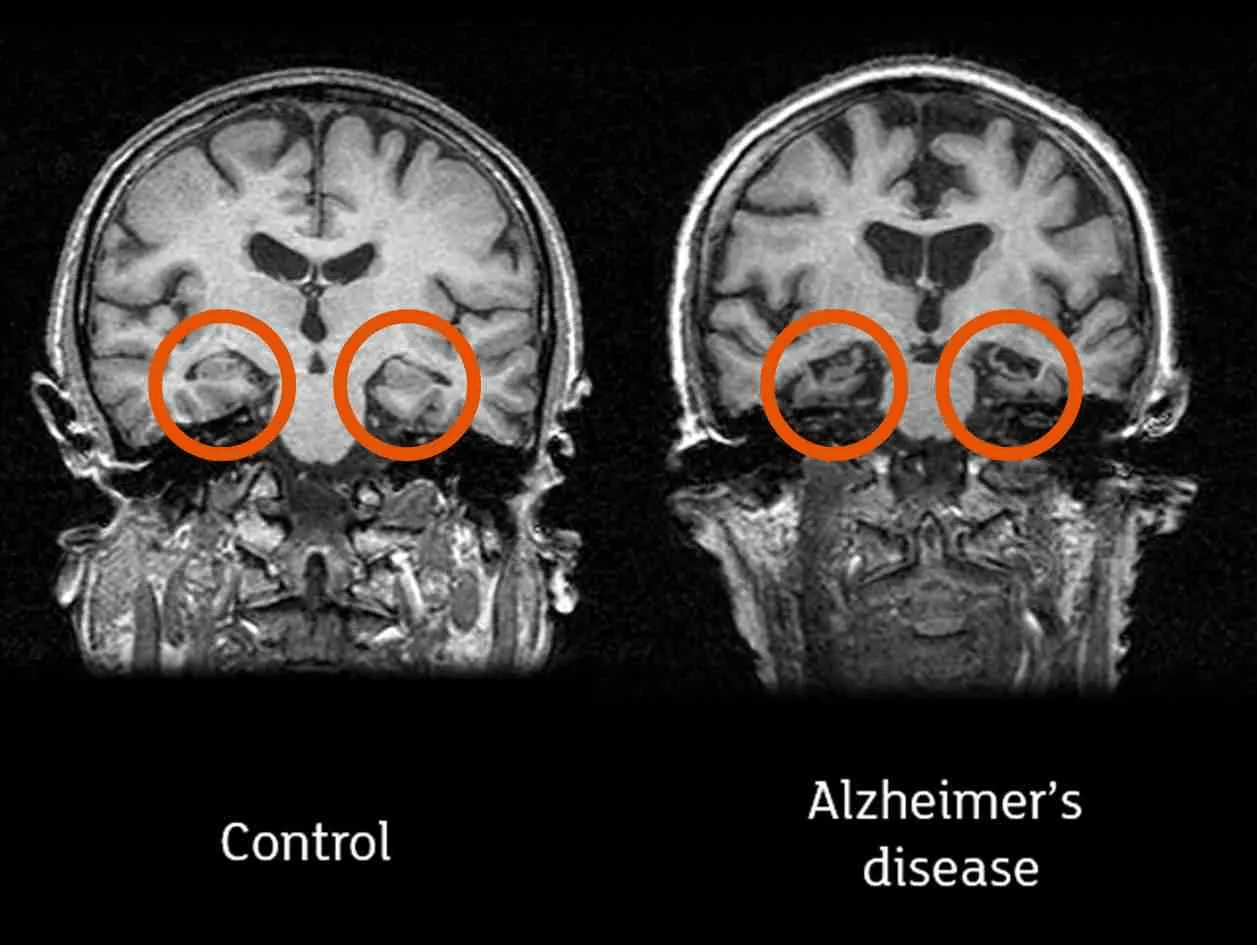
\includegraphics[width=0.8\columnwidth]{figures/fig1.png}  % Adjust the width to your liking
    \caption{Comparison of a normal brain (left) and an Alzheimer's patient's brain (right).\\Images credit: Professor John O'Brien, University of Cambridge and Newcastle University} % Caption for the image
    \label{fig:alzheimers_brain} % Label to reference the image later in the document
\end{figure}

A person with Alzheimer's disease will not be aware that he might be having a disease can ultimately lead to be a very dangerous disease. This is because the symptoms of Alzheimer's are very hard to find. It can be different to different people. The person can still do all the regular chores he does day to day without any problems. Having said that there will be some problems he might be facing while doing these activities, like for example not able to remember words, or not remembering names etc. People around him will definitely notice that this person has trouble remembering stuff. This is the reason why doctor as a first step usually conducts a medical interview where the person will be asked some questions. With the help of this he will be able to get a ball park idea whether he might have Alzheimer's or not. Some of the symptoms of Alzheimer's as follows,
\begin{enumerate}[nosep]
    \item Forgetting things, misplacing things, and missing meetings.
    \item Forgetting names and events.
    \item Not able to recall incidents happened in the past.
    \item Problems with audio visual memory.
    \item Being absent minded.
    \item Agitation and restlessness
\end{enumerate}

The symptoms of Alzheimer's becomes more evident when the disease progresses and one grows old. The person starts notices that the symptoms that he previously had are slowly slowly getting worse and worse. At later stages of AD it becomes very difficult to even communicate with the person as he does not remember anything. He forgets to even do the basic things that he has been taught to do since his childhood. This the stage when they will need continuous Assistance. 

\chapter{Motivation}

\begin{figure}[h!]
    \centering
    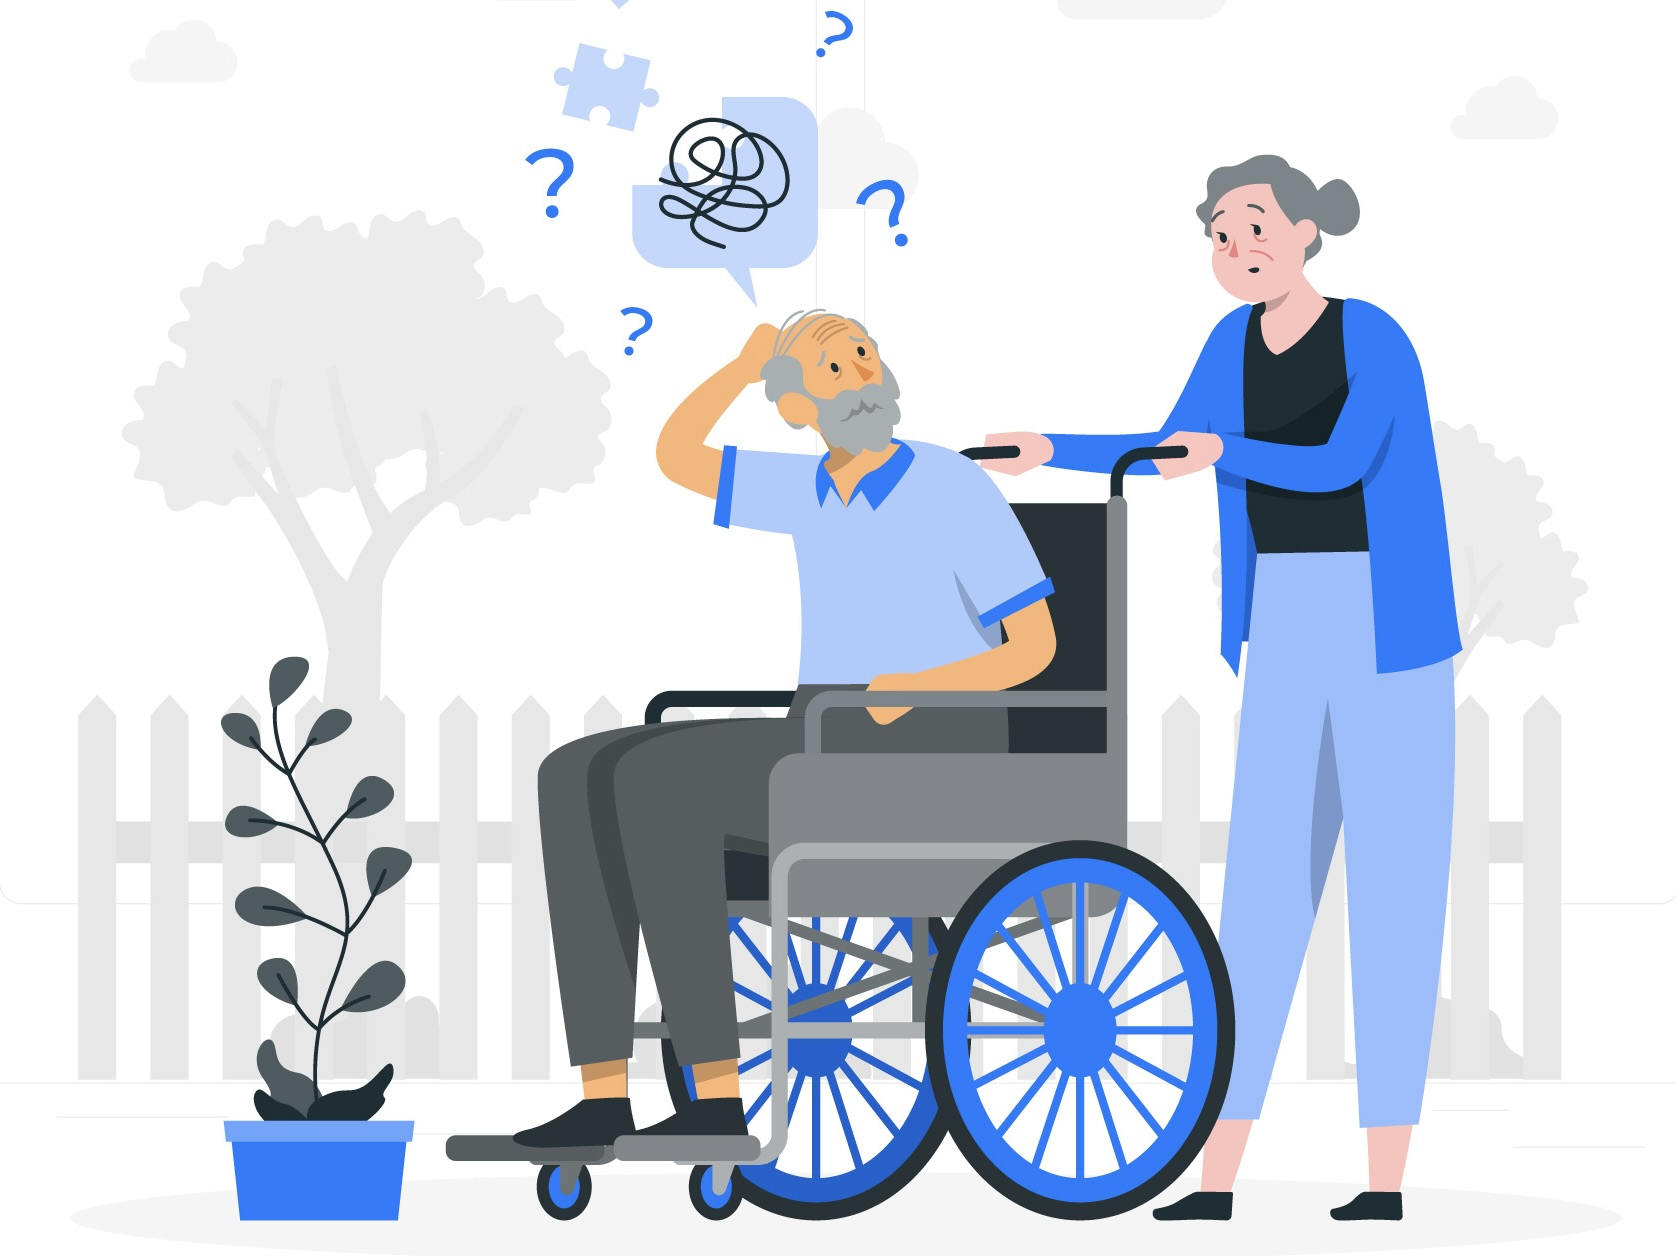
\includegraphics[width=0.8\columnwidth]{figures/fig2.jpeg}  % Adjust the width to your liking
    \caption{Person suffering from Dementia} % Caption for the image
    \label{fig:alzheimers_patient} % Label to reference the image later in the document
\end{figure}

Alzheimer's is considered as one of the most challenging disease in the modern medicine research. And this disease not only effects the individual but also impacts the people around him/her that is family, doctors and also the hospitals. As the people effected by this disease are increase at a rapid rate around us, there is a need to develop a better way to diagnose and prevent this disease. Particularly, there is a high demand for a system that will detect the disease at a early stage. So that the medical team can stop the disease from getting worse at the old age which might cause a big economic burger for the patients.

The motivation to write this thesis came from the fact that there are sophisticated diagnostics options available at the moment which are very expensive, time-consuming and they are not accessible for of people. But the main problem is even after spending a lot of money on these diagnostic procedures, it cannot detect it at a very earlier stage. Doctors use MRI's and PET scans which are very accurate but they machines used for this are very special and needs an expert to use them. Additionally, even after analyzing a persons brain in these scans, the disease is not detected at a early stage because the small changes that are happening in the brain are very different to find when compared to the normal aging of a persons brain. 

With the advanced Machine Learning techniques we can try to fix these problems that are currently there. By using the datasets that available online the advanced Machine Learning models can find patterns in the datasets which is hard to find using a naked human eyes. This will help in detecting the  Alzheimer's disease at a very earlier stage. 

Personally for me this paper is driven by the fact that I have seen many people around me struggling with Alzheimer's disease in their old age. I have seen it first hand how much time, money and effort does it take for their family to take care of them in that situation. As it is a disease that gradually gets worse, they slowly start losing their memory and identity. Having witnessed this I have seen how much effort goes into taking care of a Alzheimer's patient. This has motivated me to provide my Contribution to this communicate and make a difference. Hence, my aim in this research is to create a model will be able to predict the possibility of the disease at a earlier stage. 


\chapter{Contribution}

The contribution of this thesis paper is to use the advanced Machine Learning algorithms to find a solution to problems of early detection of the Alzheimer's disease. This is to provide a novel extension to the community of deep learning models to the Alzheimer’s stage classification.This will include implementing various different advance machine learning models to improve the predicting of the disease based on the MRI images that we are using for this research. The main contributions are such as:

\begin{enumerate}
    \item \textbf{ Inclusion of Uncertainty-Aware Framework:} In this research patient's MRI images will be analyzed which are divided into various stages of Alzheimer's and build a Classification Model using these images. Many high performing models are already presend online but in this thesis we will looking one of them and which performed the best and implement Monte Carlo Dropout Uncertainty calcucation so that the confidence of the model can be analyzed. This will help in knowing how confident the model is when predicting the class.

    \item  \textbf{ Improved Model Interpretation:} The addition made to the code to include the Uncertainty indication will help in knowing how confident the model is when predicting the classes. This will also help in the clinical environment where the professionals looking at the results of the models they will not blindly accept the stage of alzheimer's disease, they can check if the model was confident when predicting the class. If not they can furthur review with their senior doctors about the case.

    \item \textbf{ Addition of Uncertainty Score in Predicted Results:}
    In this thesis a very much necessary steps in the deep learning models when it comes to medical usage are being looked at and included. These additional metrics will ensure that models performance is not evaluated only based on the accuracy but important factors like Uncertainty or confidence is considered so that cases with high uncertainty can be taken for further studies instead of just labeling whatever the model is classifying it as. A well structure visualization framework is put into action to highlight uncertainty for each and every individual predicted images. These information on the visualization will allow clinicians to find and focus on unique and unknown cases, which will allow them to make more informed decision-making.
    

    \item \textbf{Utilization of Publicly Available Datasets:} The MRI images used for this study is a cleaned dataset which is availabel on kaggle which is sourced from ADNI websites which are the MRI images of actual people with true labels. Since it's is very reliable source this study uses real world data to train the model at the same time following all the ethical guidelines.
    
    \item \textbf{Visualization of Uncertainty in Predictions:} By focusing on machine learning approaches, the research aims to provide scalable and cost-effective solutions for early AD diagnosis. This could significantly improve accessibility, especially in resource-constrained settings where sophisticated imaging technologies are not viable.

    \item \textbf{New addition will make it possible for this to be applied in a clinical setup:} By introduction Uncertainty into account when classifying the Alzheimer’s Disease into multiple classes this thesis reseach will help reducing the rist of wrong diagnosis in a medical setup who are ready to introduce AI into for their diagnostics setup. It is especially important in medical field as misdiagnosis might cause a major problems in a persons life.

    \item \textbf{Contribution to the AD community as well as open sourcing these projects:} The code used for this thesis will be open to everyone to view and as this will allow to access and reproduce this models for further studies. By adding Uncertainty to these already well performing models this reasearch further improves the the communities acceptence of these new technologies into their system, as it also allows human proffessionals to take things into their hands the models is not so sure how to react the unexpected situations.

\end{enumerate}



\chapter{Literature Review}

In the recent years have seen a impressive amount of progress in the utilization of the deep learning models for the Alzheimer’s Disease detection based on the MRI data. And alot of advancement focus on how to improve, how accurately the model predicts the Disease of how accurately it classifies the images or data into different classes. Whereas the integration of Uncertainty calculation is something that is not explored too much, nevertheless. In this Literature review the previous research papers are being studied and will be compared and seen if there are any gaps in the study that can be full filled.

\section{Overview of techniques used on MRI}
All thanks to the impressive technology of the Magnetic Resonance Imaging(MRI), Alzheimer's disease (AD) can be detected at a very early stage compared to earlier. The 3 Dimensional high quality images of brain captured using MRI machines provide a view of our brain with which we can find the patterns in the parts of the brain like temporal regions and hippocampal region which helps in diagnose of the Alzheimer’s Disease. By taking a look at the white matter integrity and functional connectivity, the help of diffusion tensor imaging (DTI) and functional magnetic resonance imaging (fMRI) make amazing contributions to this. Methods such as cortical thickness measurement and voxel-based morphometry have been widely used for quantitative analysis of structural changes and brain volume\cite{zou2023}.

Recently, there have been studies that are going on to create synthetic longitudinal MRI images for Alzheimer's disease using a conditional diffusion model. Diffusion models are are excellent at producing high-quality images with consistent training, which are used in this strategy. The models can produce realistic target pictures that mimic the course of the disease by using the time interval and the source MRI scan as conditioning elements. This strategy may be able to get around the drawbacks of current techniques like GANs and VAEs, which can have unstable, undiversified, or hazy results. The suggested model offers a useful tool for Alzheimer's disease research and clinical applications, producing high-fidelity synthetic MRI scans with encouraging findings\cite{Duy2024}.


\section{Using Deep Learning for Alzheimer’s Detection}
The most common type of dementia that causes a lot of trouble for  millions of people worldwide is Alzheimer's disease (AD). In order to manage symptoms and maybe reduce the progression of the disease, early recognition of AD is essential\cite{2023ShenLiu}.Conventional diagnosis techniques depend on radiologists' subjective and time-consuming manual review of brain imaging data. And that is where Deep Learning brings an serious advantage over the time consuming tasks. Deep Learning models can predict these kind of tasks with the mater of seconds.

With the use of deep neural networds we have see an amazing results in the recent years. Using the MRI data, and deep learning neural networks in prediction of the early detection of the Alzheimer’s Disease has been a very promision method with great acccuracy. The convolutional neural networks as well as the recurrent neural netword have have drastically improve the prediction for this desease when compared to the traditionaL Machine Learning alternatives. This is because the Deep Learning models are able undertand the complex nature of the high dementional data that are used in training these models and to capture the brain image\cite{2019Jo}. Recent improvements in the this field, specially deep leaning have changed the landscape of the Alzheimer’s Detection. It is able to provide an objective and efficient solution.

Convolutional Neural Networks (CNNs) is a kind of deep learning model which has showed the world it's abilities with great results in prediction of Alzheimer’s with the help of MRI images. Very high resolution images or high dimensional data's can be trained using these models, which will find the existing patters in these data, and helps in detecting Alzheimer’s at a very early stage. By drastically reducing the time and efforts required in the diagnosis process of the Alzheimer’s Disease and being able to predict with great precision,these deep learning models perform impressively better than than the conventional machine learning models.


Let's check some of the recent studies. The summary of the studies is provided in the Table~\ref{tab:methods_comparison} :
\begin{table*}[h!]
    \centering
    \caption{Comparison of Studies on Alzheimer’s Disease Detection}
    \label{tab:methods_comparison}
    \begin{tabular}{|p{3cm}|p{3cm}|p{3cm}|p{2cm}|p{4cm}|}
        \hline
        \textbf{Study} & \textbf{Dataset} & \textbf{Model} & \textbf{Accuracy} & \textbf{Limitations} \\ \hline
        Sharma, Sarang (2022) \cite{2022Sarang} & Kaggle & Hybrid Deep Learning Model & 91.75\% & No uncertainty estimation, limited interpretability \\ \hline
        Desai, Maitri (2024) \cite{2024Desai} & OASIS & Multi-Task CNN & 91.0\% & Limited generalizability, lacks uncertainty \\ \hline
        Ahmed, Gulnaz (2022) \cite{2022Ahmed} & OASIS & DAD-Net & 99.22\% & No reliability or uncertainty analysis \\ \hline
        Sarraf et al. (2016) \cite{sarraf2016} & ADNI & CNN (LeNet-5) & 98.84\% & High false negatives \\ \hline
        Farhana Islam et al. (2023) \cite{Islam2023} & Custom MRI Dataset & ResNet-50 & 98.71\% & No uncertainty estimation \\ \hline
        Santos et al. (2023)  \cite{Santos2023} & Kaggle & Neural Network & 80.6\% & Moderate accuracy, lacks optimization \\ \hline
        El-Latif et al. (2023) \cite{Latif2023} & Kaggle & Lightweight Deep Learning Model & 95.9\% & No uncertainty quantification \\ \hline
        Isunuri et al. (2023) \cite{Isunuri2023} & Kaggle & Transfer Learning with CNN & 97.32\% & Limited interpretability \\ \hline
        Murugan et al. (2023) \cite{Murugan2021} & Kaggle & DEMNET & 95.23\% & No uncertainty assessment \\ \hline
        Gupta et al. (2023) \cite{Gupta2019} & NRC Korea & DEMNET & 96.89\% & No reliability metrics \\ \hline
    \end{tabular}
\end{table*}

In recent studies, various different techniques have been used to predict the alzheimers disease. Out of all of them deep learning models have shows a lot of potential and promise with great results. Deep learning is widely used acrross various fields or study, but the stream where we excel the most is classification of the images. As in recent times people are able to get hands on the powerful hardware as it has become accessible, and more research are being conducted on Deep Learning models there has been alot of improvement in the performance and hence the reliability of these models have been increased \cite{Yu2023}.
Particularly for alzheimer's there have been several studied that have been conducted. In this study we will be looking at few of them. In a paper by Sharma et al. \cite{2022Sarang} they propose HTLML. It is a hybrid deep learning model that uses the Kaggle dataset to predict the Alzheimer’s Disease. In their implementations they were able to achieve an accuracy of 91.75\%. Which is a very good performace. But what it lacks is the implementation of uncertainty estimation. When it comes to a clinical environment it would be very advantageous for clinicians to know how confident the model is. The lack of uncertainty estimation is a rather common gap found in many existing studies, limiting them to consider for a clinical deployment.In the reseach conducted by Desai et al. \cite{2024Desai}, they use a Multi-Task CNN model using the OASIS dataset to diagnose Alzheimer’s. Their model achieved an accuracy of 91.0\%, but limitations of the model is it's generalizability. The authors themselves mention in the paper that the model performs good on the OSIS dataset but it might struggle to perform well in the real-world clinical data. Generalizability is considered to be a very common issue with the deep learning models. Specially when there is not enough data to be trained on or there is no diverse patient data. Or when tested to perform with the real world data. In a paper by author Ahmed et al. \cite{2022Ahmed} has experimented with DAD-Net, it is also a deep learning-based model for Alzheimer’s detection. Here they have used ADASYN to oversample the data as the dataset they used was imbalanced. Using the deep leaning network they managed to get an impressive accuracy of 99.22\%. This model again however does not incorporate Uncertainty calcucation. Even through the model prediction is high, without the model confidence/ Uncertainty implementation it's implementation in a clinical environment will be very low because even when the model is struggling the clinicians needs to know it so that they can take a informed desicion. the model does not incorporate uncertainty estimation, which is a crucial factor for clinical decision-making. While the high accuracy is promising, the lack of uncertainty estimation limits the model's applicability in high-stakes environments such as healthcare.
Sarraf et al. \cite{sarraf2016} use CNNs and LeNet-5 for the classification of Alzheimer’s classification with the ADNI image dataset. They achieved an accuracy of 98.84\%. However, the study is criticized for its high false-negative rate, which can lead to misdiagnosis in clinical applications. Additionally, this work does not include any discussion of uncertainty estimation, further limiting its clinical relevance. Islam et al. \cite{Islam2023} proposed a method using the ResNet50 feature extractor and an SVM classifier for diagnosing Alzheimer’s disease from MRI images. This study achieved an accuracy of 98.71\%, but it lacked assessment of the model reliability. Since there is no assessment with the unseen data the reliablity of the model is hard to know with the real world data. Even in this paper the Uncertainty calcucation is not considered. Further in the study of neural network model for Alzheimer’s prediction by Santos et al. \cite{Santos2023}, they employed a neural network model on  the Kaggle dataset, and were able to get a accuracy of 80.6\%. While the model is able to provide the diagnosis and classification the performance of the model could be improved compared to other models. In the conclusion the authors suggested that the model could be improved through further research, but uncertainty estimation is not part of their investigation, which is a limitation. El-Latif et al. \cite{Latif2023} presented a very lightweight deep learning model for Alzheimer’s disease detection using MRI data. The model achieved an accuracy of 95.9\%, but like the previous case the authors acknowledged that the performance could be improved further. Again the lack of uncertainty estimation is a limitation. Isunuri et al. \cite{Isunuri2023} employ transfer learning and a CNN for Alzheimer’s severity classification, achieving an accuracy of 97.32\%. Even though the model demonstrates very good performance performance, there is no mention of uncertainty estimation, which could add a layer of reliability and interpretability to the model’s predictions. The authors also note that the model outperforms competing models in several metrics, yet its generalizability to other datasets is unclear.
Murugan et al. \cite{Murugan2021} introduced DEMNET, again it a type of deep learning model itself for the sake of early diagnosis of Alzheimer’s disease from MRI images. The model achieved an accuracy of 95.23\%, but the authors acknowledged that the performance of the model could have been be improved. While the model is promising, it does not incorporate uncertainty estimation, which is a critical aspect for clinical use as earlier mentioned where decisions based on model predictions can have serious consequences. Gupta et al. \cite{Gupta2019} use combined features from voxel-based morphometry and cortical, subcortical, and hippocampus regions of MRI T1 brain images for early Alzheimer’s diagnosis. With an accuracy of 96.89\%, the study demonstrates a robust method for Alzheimer’s detection. But similar to other studies, it lacks a mechanism for assessing uncertainty, which is important for practical deployment in healthcare environments.

\section{Limitations of Existing Approaches}
Table \ref{tab:methods_comparison} all the previous existing papers and research have been summarized, it also highlights the study's limitations. Many papers and research have models that do exceptionally well with accuracy, but then all the paper lacks the attempt to include uncertainty score as an output which might turn out to be invaluable and crucial in a clinical environment in decision-making. Furthermore, some of the models had issues with high false-negative rates, less generalizability, and dataset bias still exists. These problems support a requirement or necessity for the inclusion of uncertainty estimation so that the clinical usability and reliability of the model can be improved. When the stakes are high in clinical settings, it is challenging to trust models that lack uncertainty measurements. Adding uncertainty estimates to deep learning models can improve their interpretability and give medical professionals important information about the accuracy of the model's predictions. By using uncertainty-aware deep learning to enhance the applicability of Alzheimer's diagnosis models, this study fills a significant gap in the body of existing literature.


\section{Novelty of the Proposed Approach}
The integration of uncertainty estimation into deep learning models addresses critical gaps in existing research. By providing confidence scores alongside predictions, clinicians can make informed decisions, reducing the risks associated with false negatives or overfitting to biased datasets. This approach also enhances model interpretability, a vital factor for clinical adoption.



\chapter{Methodology}

In this chapter the methedology used in this thesis for training, developing, evaluating and developing an uncertainty-aware deep learning model will be discussed. This sections will be taking you into the deep dive into why certain things are choosen over others. Each and every step from the loading of the dataset, data augmentation, model building, evaluation metrics, uncertainty awareness in the model and as well building an web application to predict Alzheimer's which can be used in a clinical environment.

\section{Dataset used for this research}

\subsection{About Dataset}

\begin{figure}[h!]
    \centering
    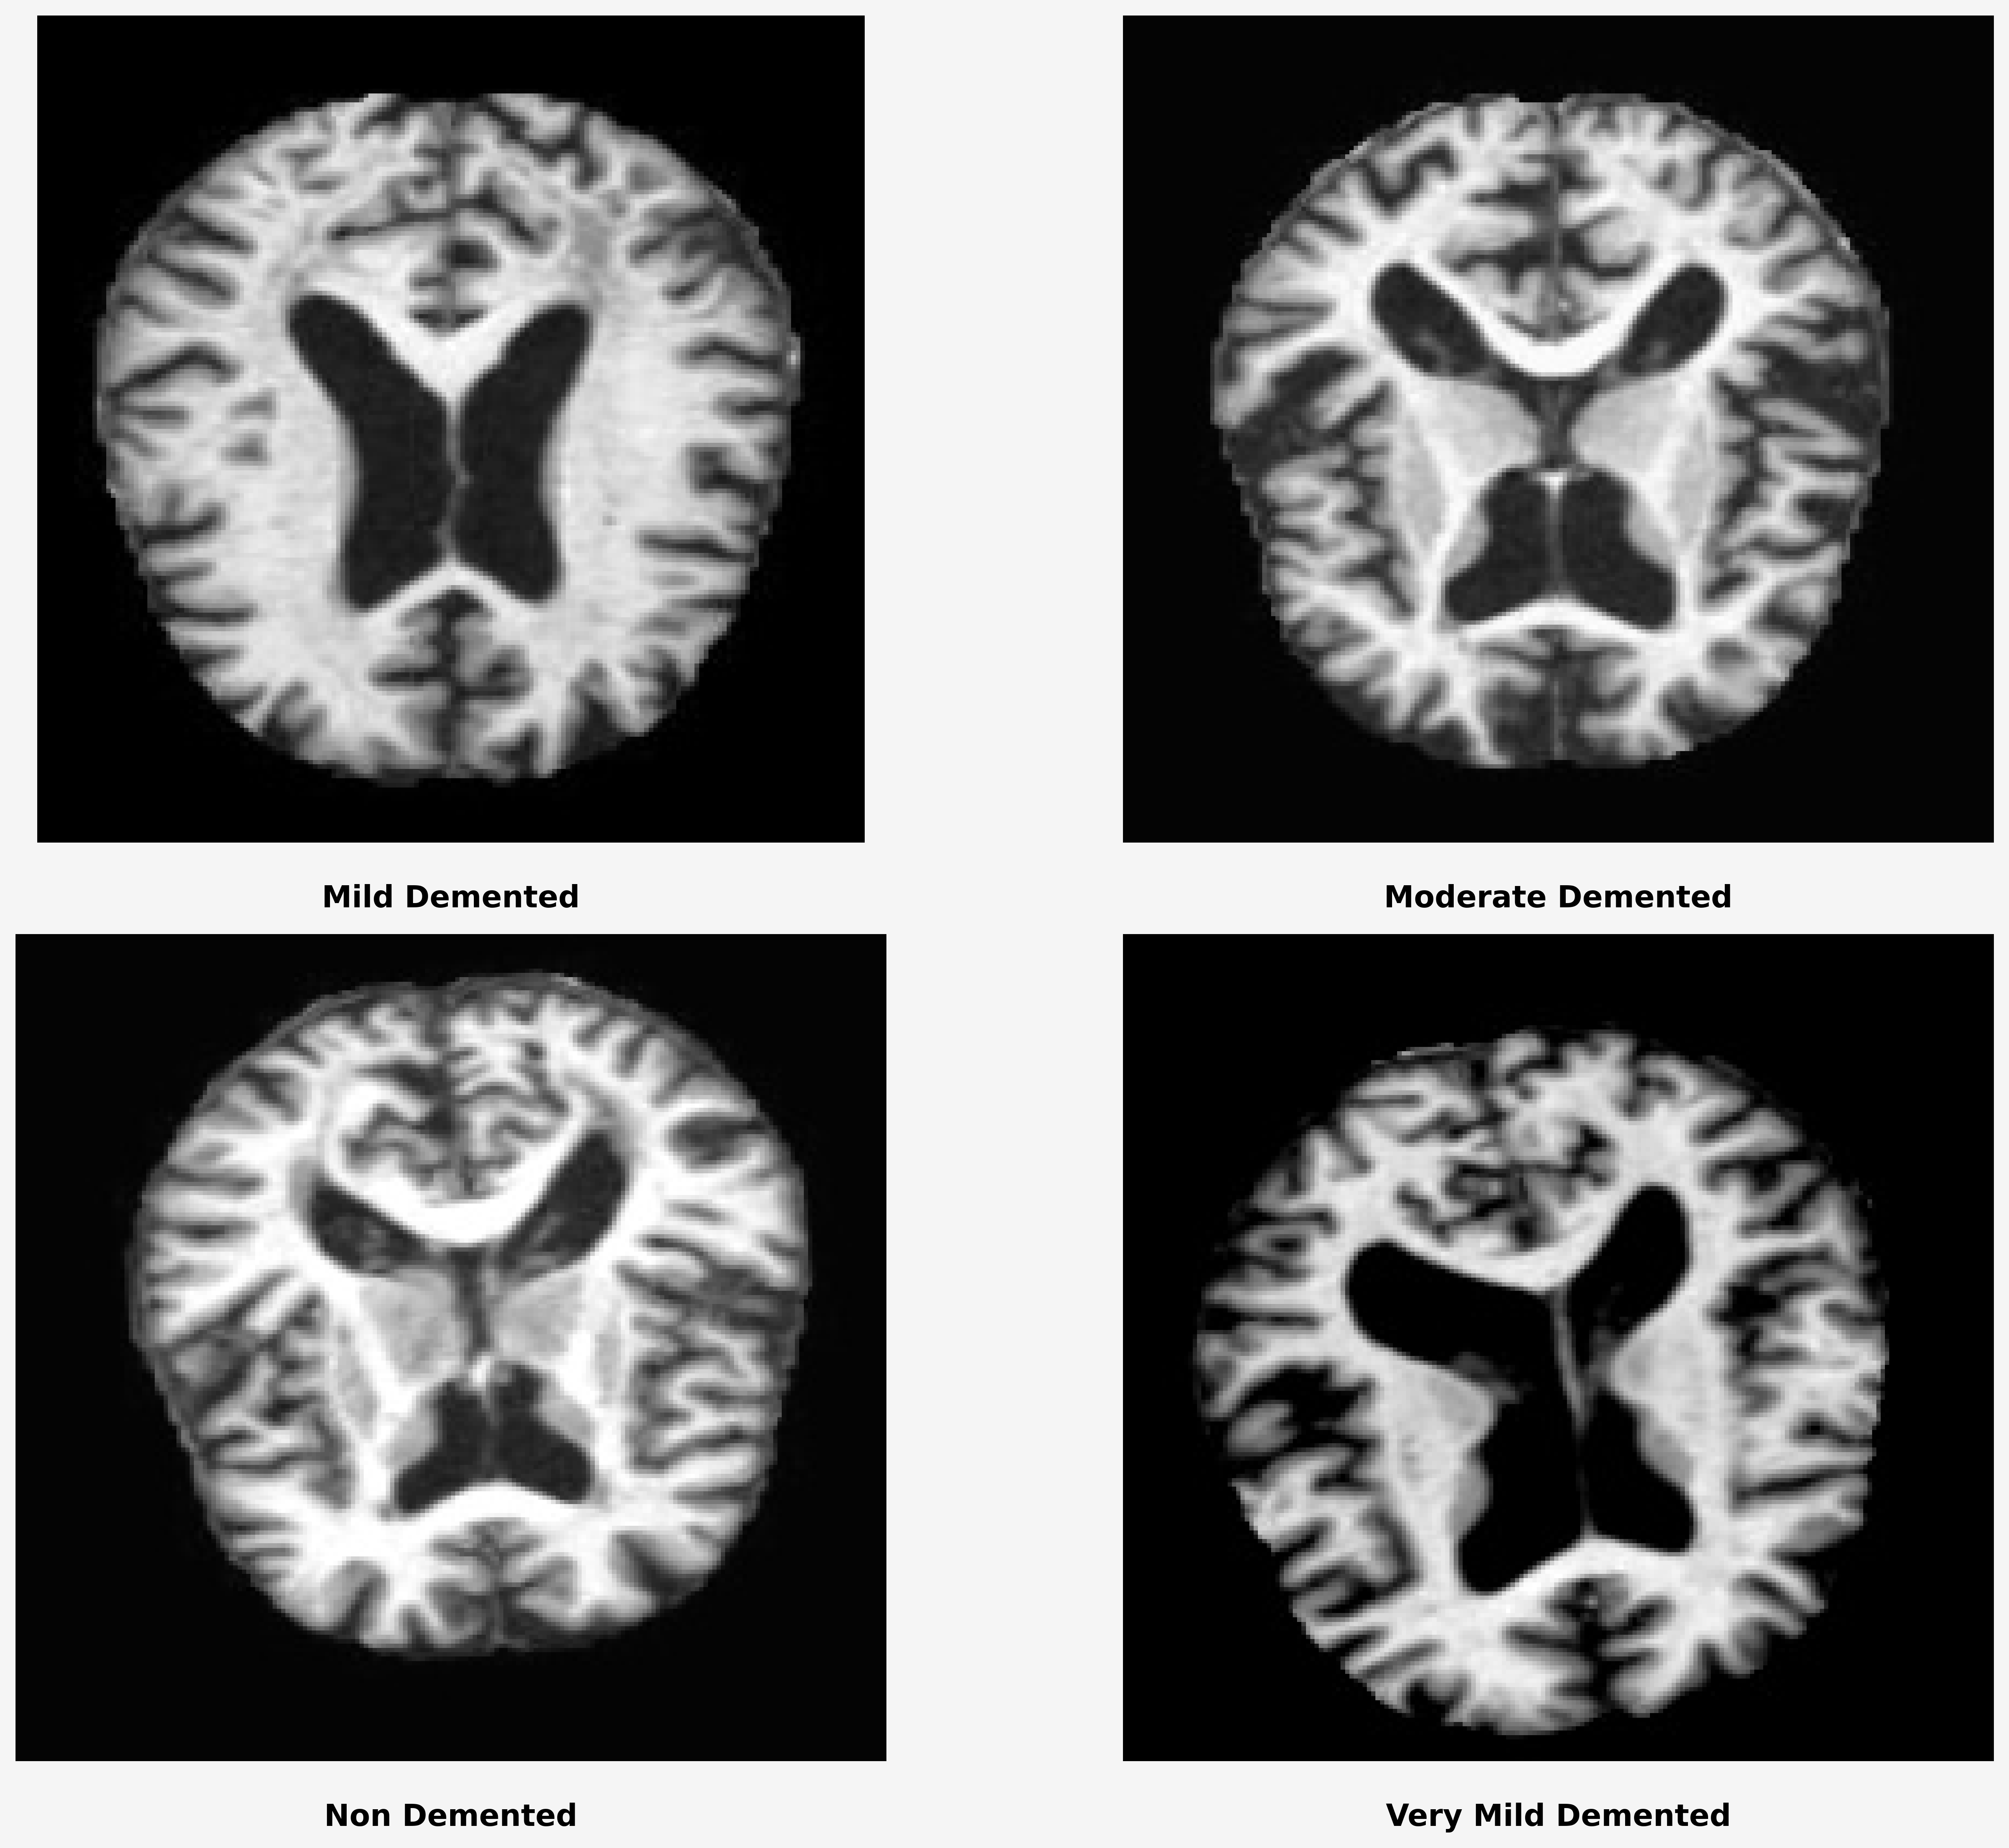
\includegraphics[width=0.8\columnwidth]{figures/dataset.png}  % Adjust the width to your liking
    \caption{Sample images of the dataset} % Caption for the image
    \label{fig:dataset} % Label to reference the image later in the document
\end{figure}

For this study the dataset used from a publicly available dataset. The dataset is availabel here \url{https://www.kaggle.com/datasets/uraninjo/augmented-alzheimer-mri-dataset}. This dataset is derived from the MRI dataset that is available on the ADNI website \url{https://adni.loni.usc.edu/}. This dataset consists of high quality 2D Magnetic Resonance imaging(MRI) scans images. Magnetic Resonance imaging scans are usually 3D, but this particular images dataset that is availabel on Kaggle is being processed and converted into high quality 2D images. This dataset is best suited for multi class classification task. The images are being divided into 4 different classes based on the stages of the alzheimer's the patients are in. And the folder names are the true labels of the images:
\begin{enumerate}
    \item \textbf{NonDemented} – This consits of MRI images of brains which does not show any sign of having Alzheimer’s Diseace or in other words cognitive impairment. There are a total of 9600 images of the Non Demeted brains in this dataset.
    \item \textbf{VeryMildDemented} – This consists of MRI images of the brains which shows slight early sign's of patient progressing towards Alzheimer’s Disease. There are a total of 8960 images of the Very Mild Demented brains in this dataset.
    \item \textbf{MildDemented} – This consists of MRI images of the brains which show mild structural brain changes of patient progressing towards Alzheimer’s Disease. These patients will start having noticeable memory problems and cognitive problems. There are a total of 8960 images of the Mild Demented brains in this dataset.
    \item \textbf{ModerateDemented} – This consists of MRI images of the brains which shows significant structural brain changes of patient Alzheimer’s Disease. This is a advanced stage of the Alzheimer’s disease. These patients will start having noticeable memory problems and cognitive problems as well. There are a total of 6464 images of the Mild Demented brains in this dataset.
\end{enumerate}


\subsection{Dataset Features}
Let's look at the features of the dataset that is used for this paper. There are two set's of images data in this dataset. One is the original images and the second one is the augmented images. For this research we will be taking Augmented images as the base models that we are taking from the Kaggle source has used this dataset. Hence we will be using this. The images are divided into 4 classes and images of each classes are placed in their on Folder's namely, NonDemented, VeryMildDemented, MildDemented and ModerateDemented.
\begin{enumerate}
    \item \textbf{Size of Dataset} 
    – The total size of the dataset is 366 megabytes. It consists of thousands of high quality 2 dimensional images for each classes. Which makes this dataset a perfect fit for the building a machine learning models by training the model using these real world datasets.
    \item \textbf{Dimensions of the Dataset} – The original images of this datasets roots from the collection of MRI images from ADNI dataset. These images are originally 3 Dimensional. Having said that the dataset used for thesis are the processed images of the ADNI dataset. The images have been processed to convert to 2 Dimensional images. This helps to reduce the complexity of the model.
    \item \textbf{Class balance} 
    \begin{figure}[h!]
        \centering
        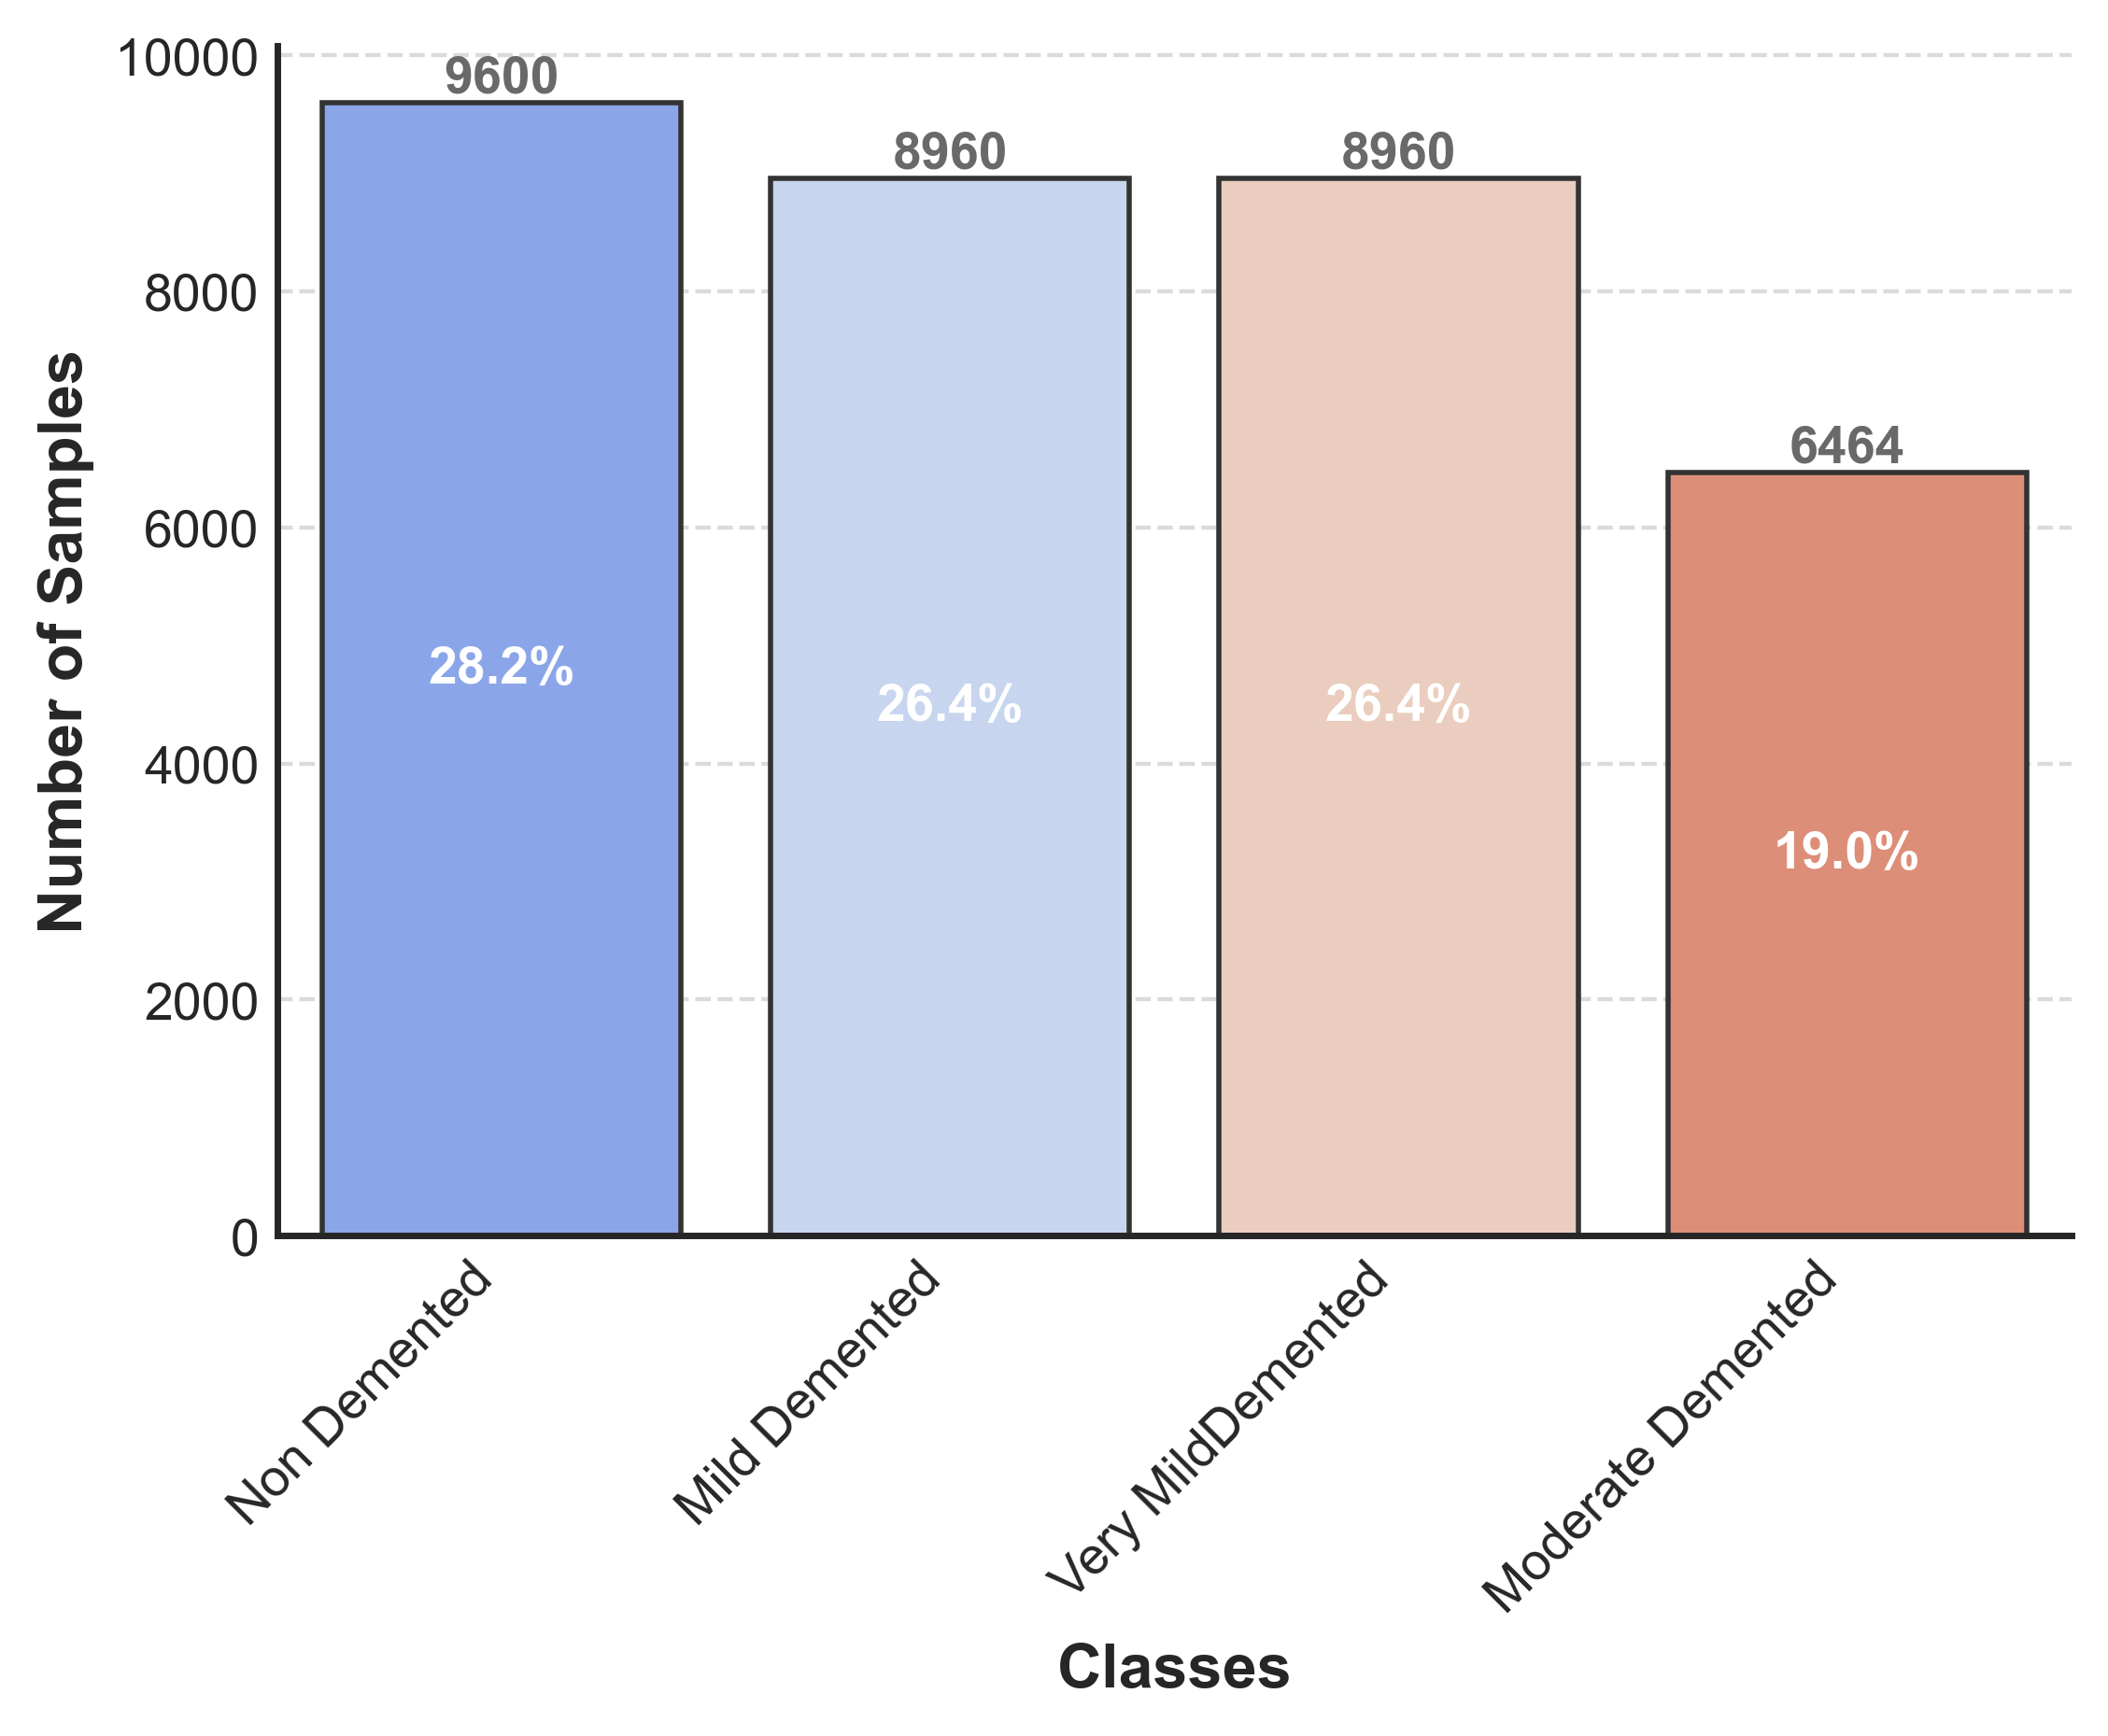
\includegraphics[width=0.8\columnwidth]{figures/dataset_class_distribution.png}  % Adjust the width to your liking
        \caption{Dataset Class distribution} % Caption for the image
        \label{fig:dataset_class_distribution} % Label to reference the image later in the document
    \end{figure}
    – The figure \ref{fig:dataset_class_distribution} shows the class distribution in the dataset. As you can see in the figure \ref{fig:dataset_class_distribution} there 9600 images for Non Demented Class, and 8960 images for Mild Demented and Very Mild Demented Class and 6464 images for Moderately Demented Class. It is a moderately imbalanced dataset. But since we are going to check for accuracy scores for each classes we are not going to balance this dataset.
    \item \textbf{Dataset Format} – Originally the ADNI datasets are stored in NIfTI format. But the Kaggle dataset that we are using is being preprocessed and saved in 2D format, all the images are stored in JPG format.
\end{enumerate}

\subsection{Ethical and Legal Considerations}
This research used a publicly available Kaggle dataset for Alzheimer’s disease detection, which strictly adheres to its licensing terms and conditions. The dataset used in this thesis is already anonymized by its authors which complies with data privacy and confidentiality standards by excluding personally identifiable information. Ethical considerations, including fairness, transparency, and interoperability, were of highest priority when designing the model. The use of Kaggle data aligns with non-commercial academic purposes, and proper attribution to the dataset’s creators is provided. No new data was collected for this study.

\section{Pre-Processing the Dataset}
\begin{figure}[h!]
    \centering
    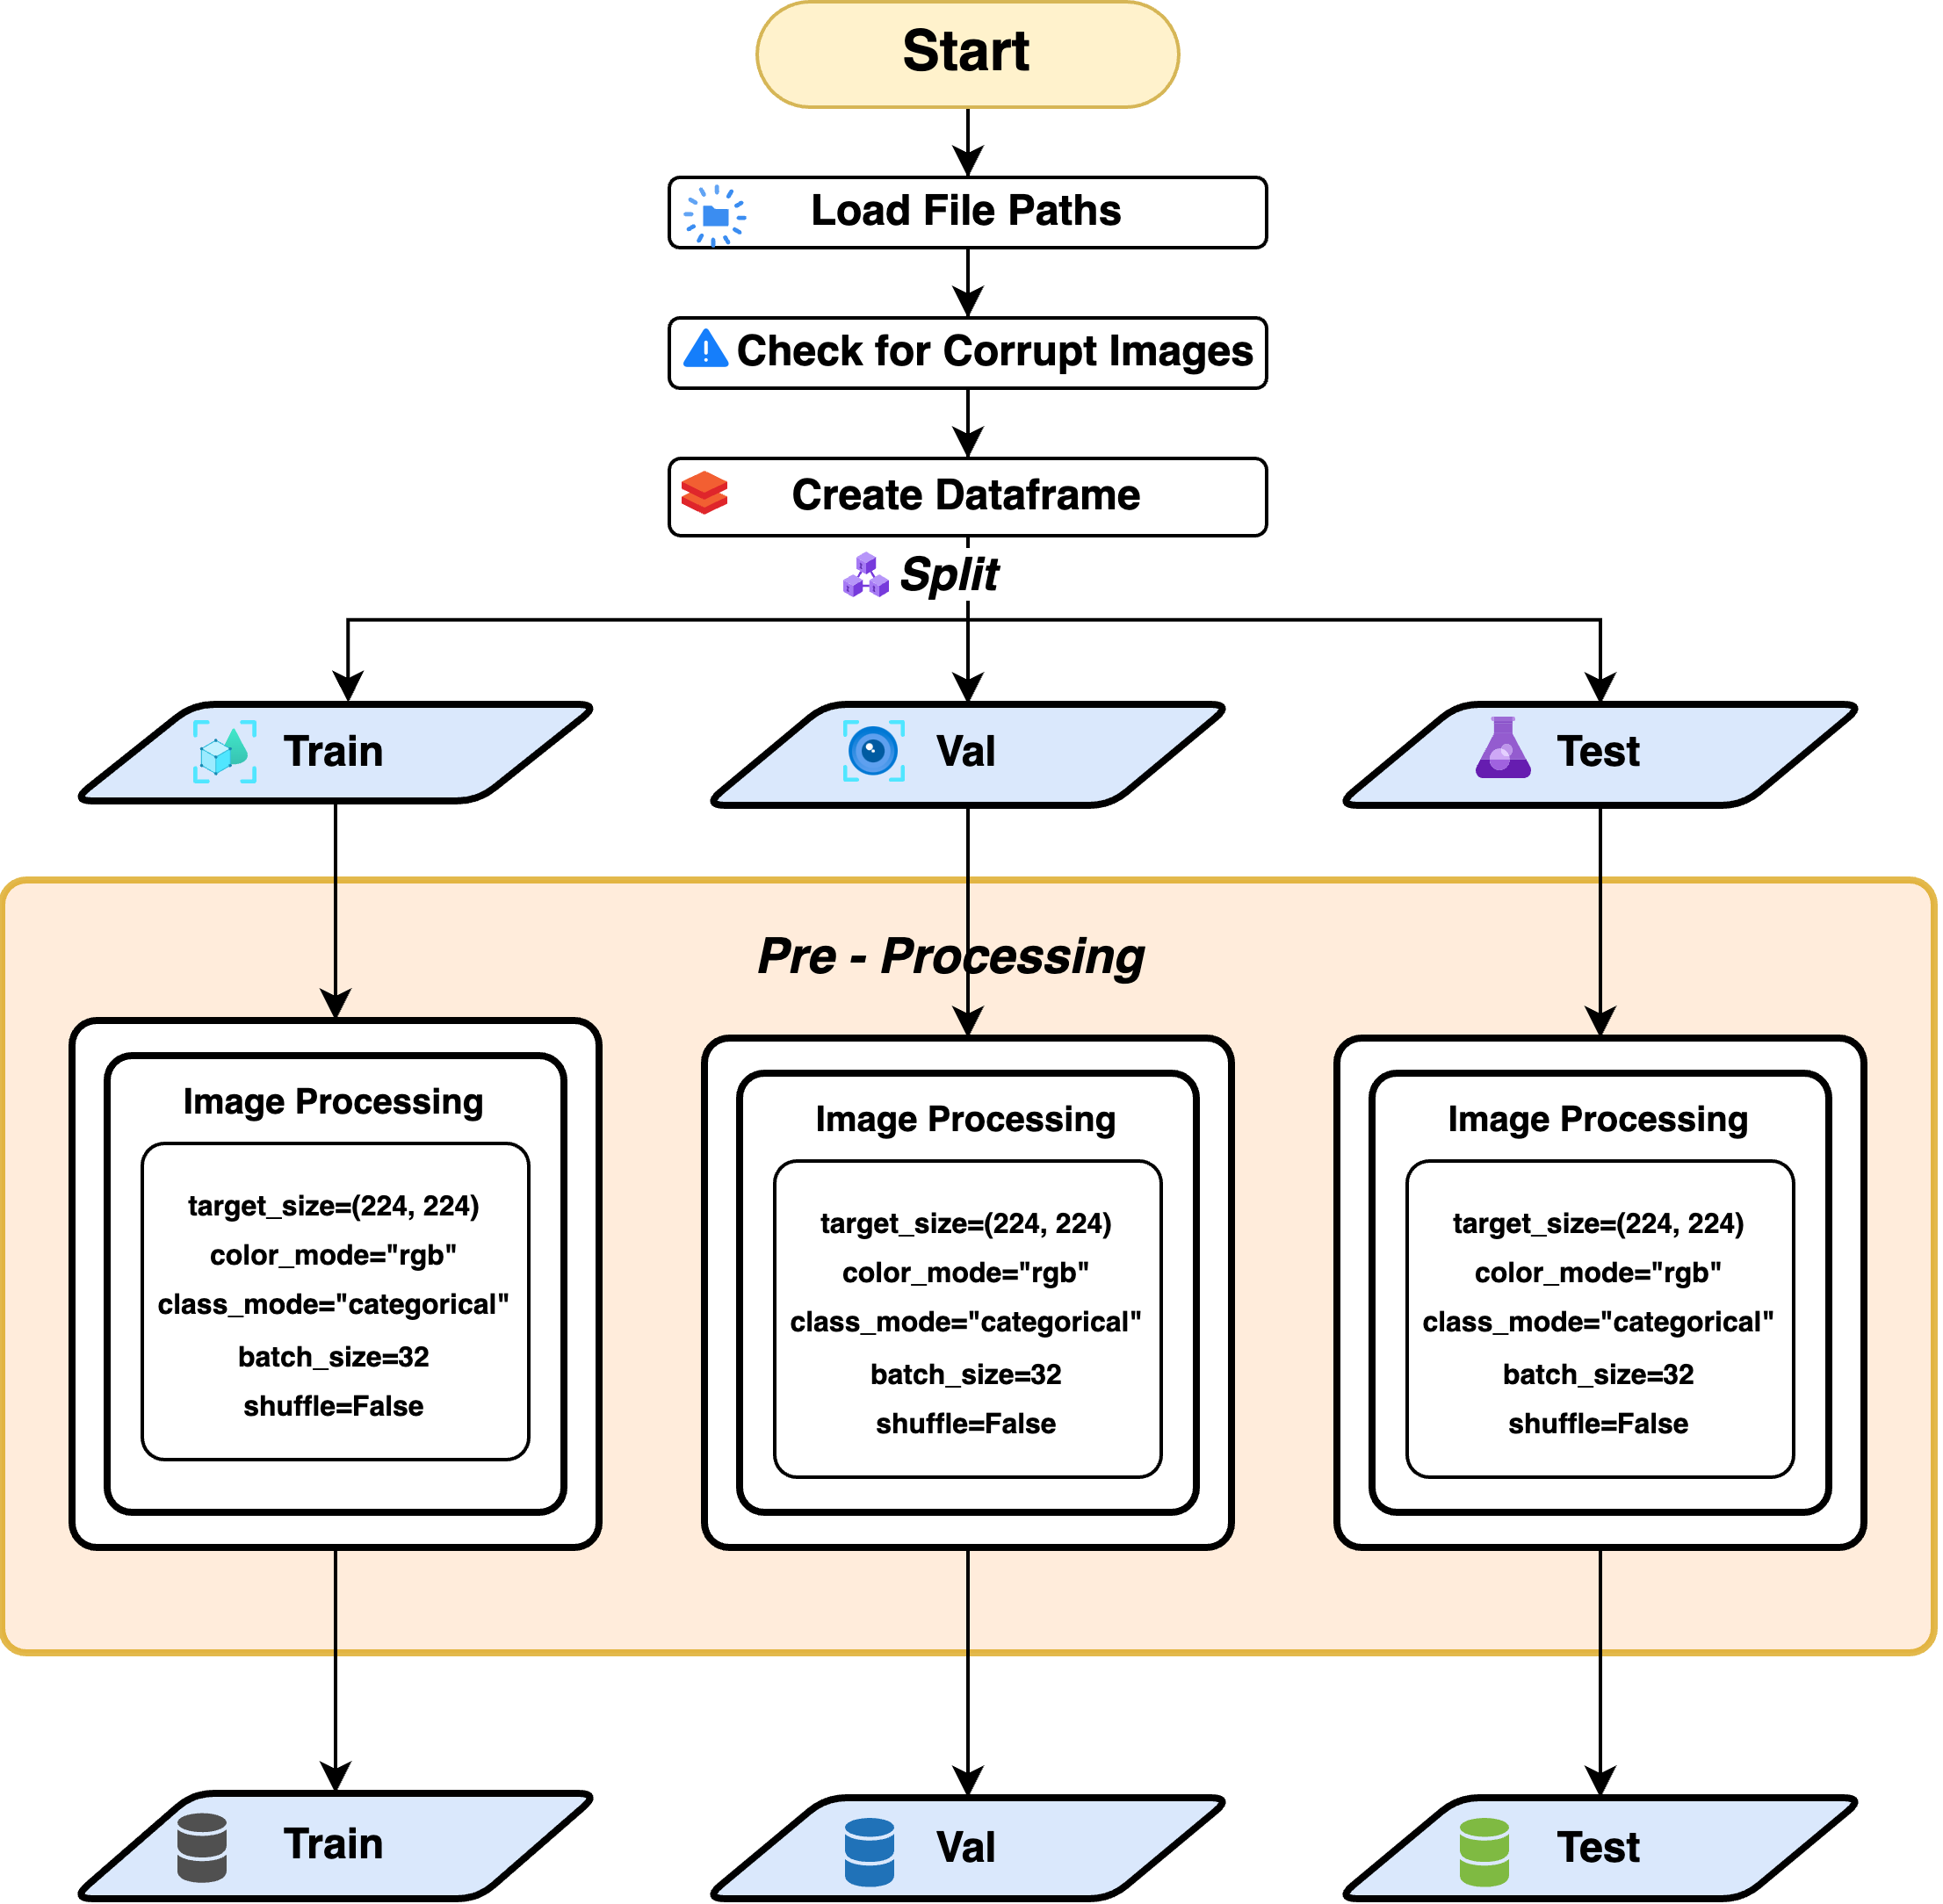
\includegraphics[width=0.8\columnwidth]{figures/image_preprocessing_full.png}  % Adjust the width to your liking
    \caption{pre-processing flow} % Caption for the image
    \label{fig:image_preprocessing_full} % Label to reference the image later in the document
\end{figure}

In order for the model to learn from the patterns in the images it is very import that the images are being processed properly. Data is processed so that the model can learn from it in a efficient and effective way. Figure \ref{fig:image_preprocessing} shows the steps applied on the images so that it can compatible with the model, and read as much details as possible but at the same time be efficient in learning from it.

\subsection{Data Cleaning}
\begin{figure}[h!]
    \centering
    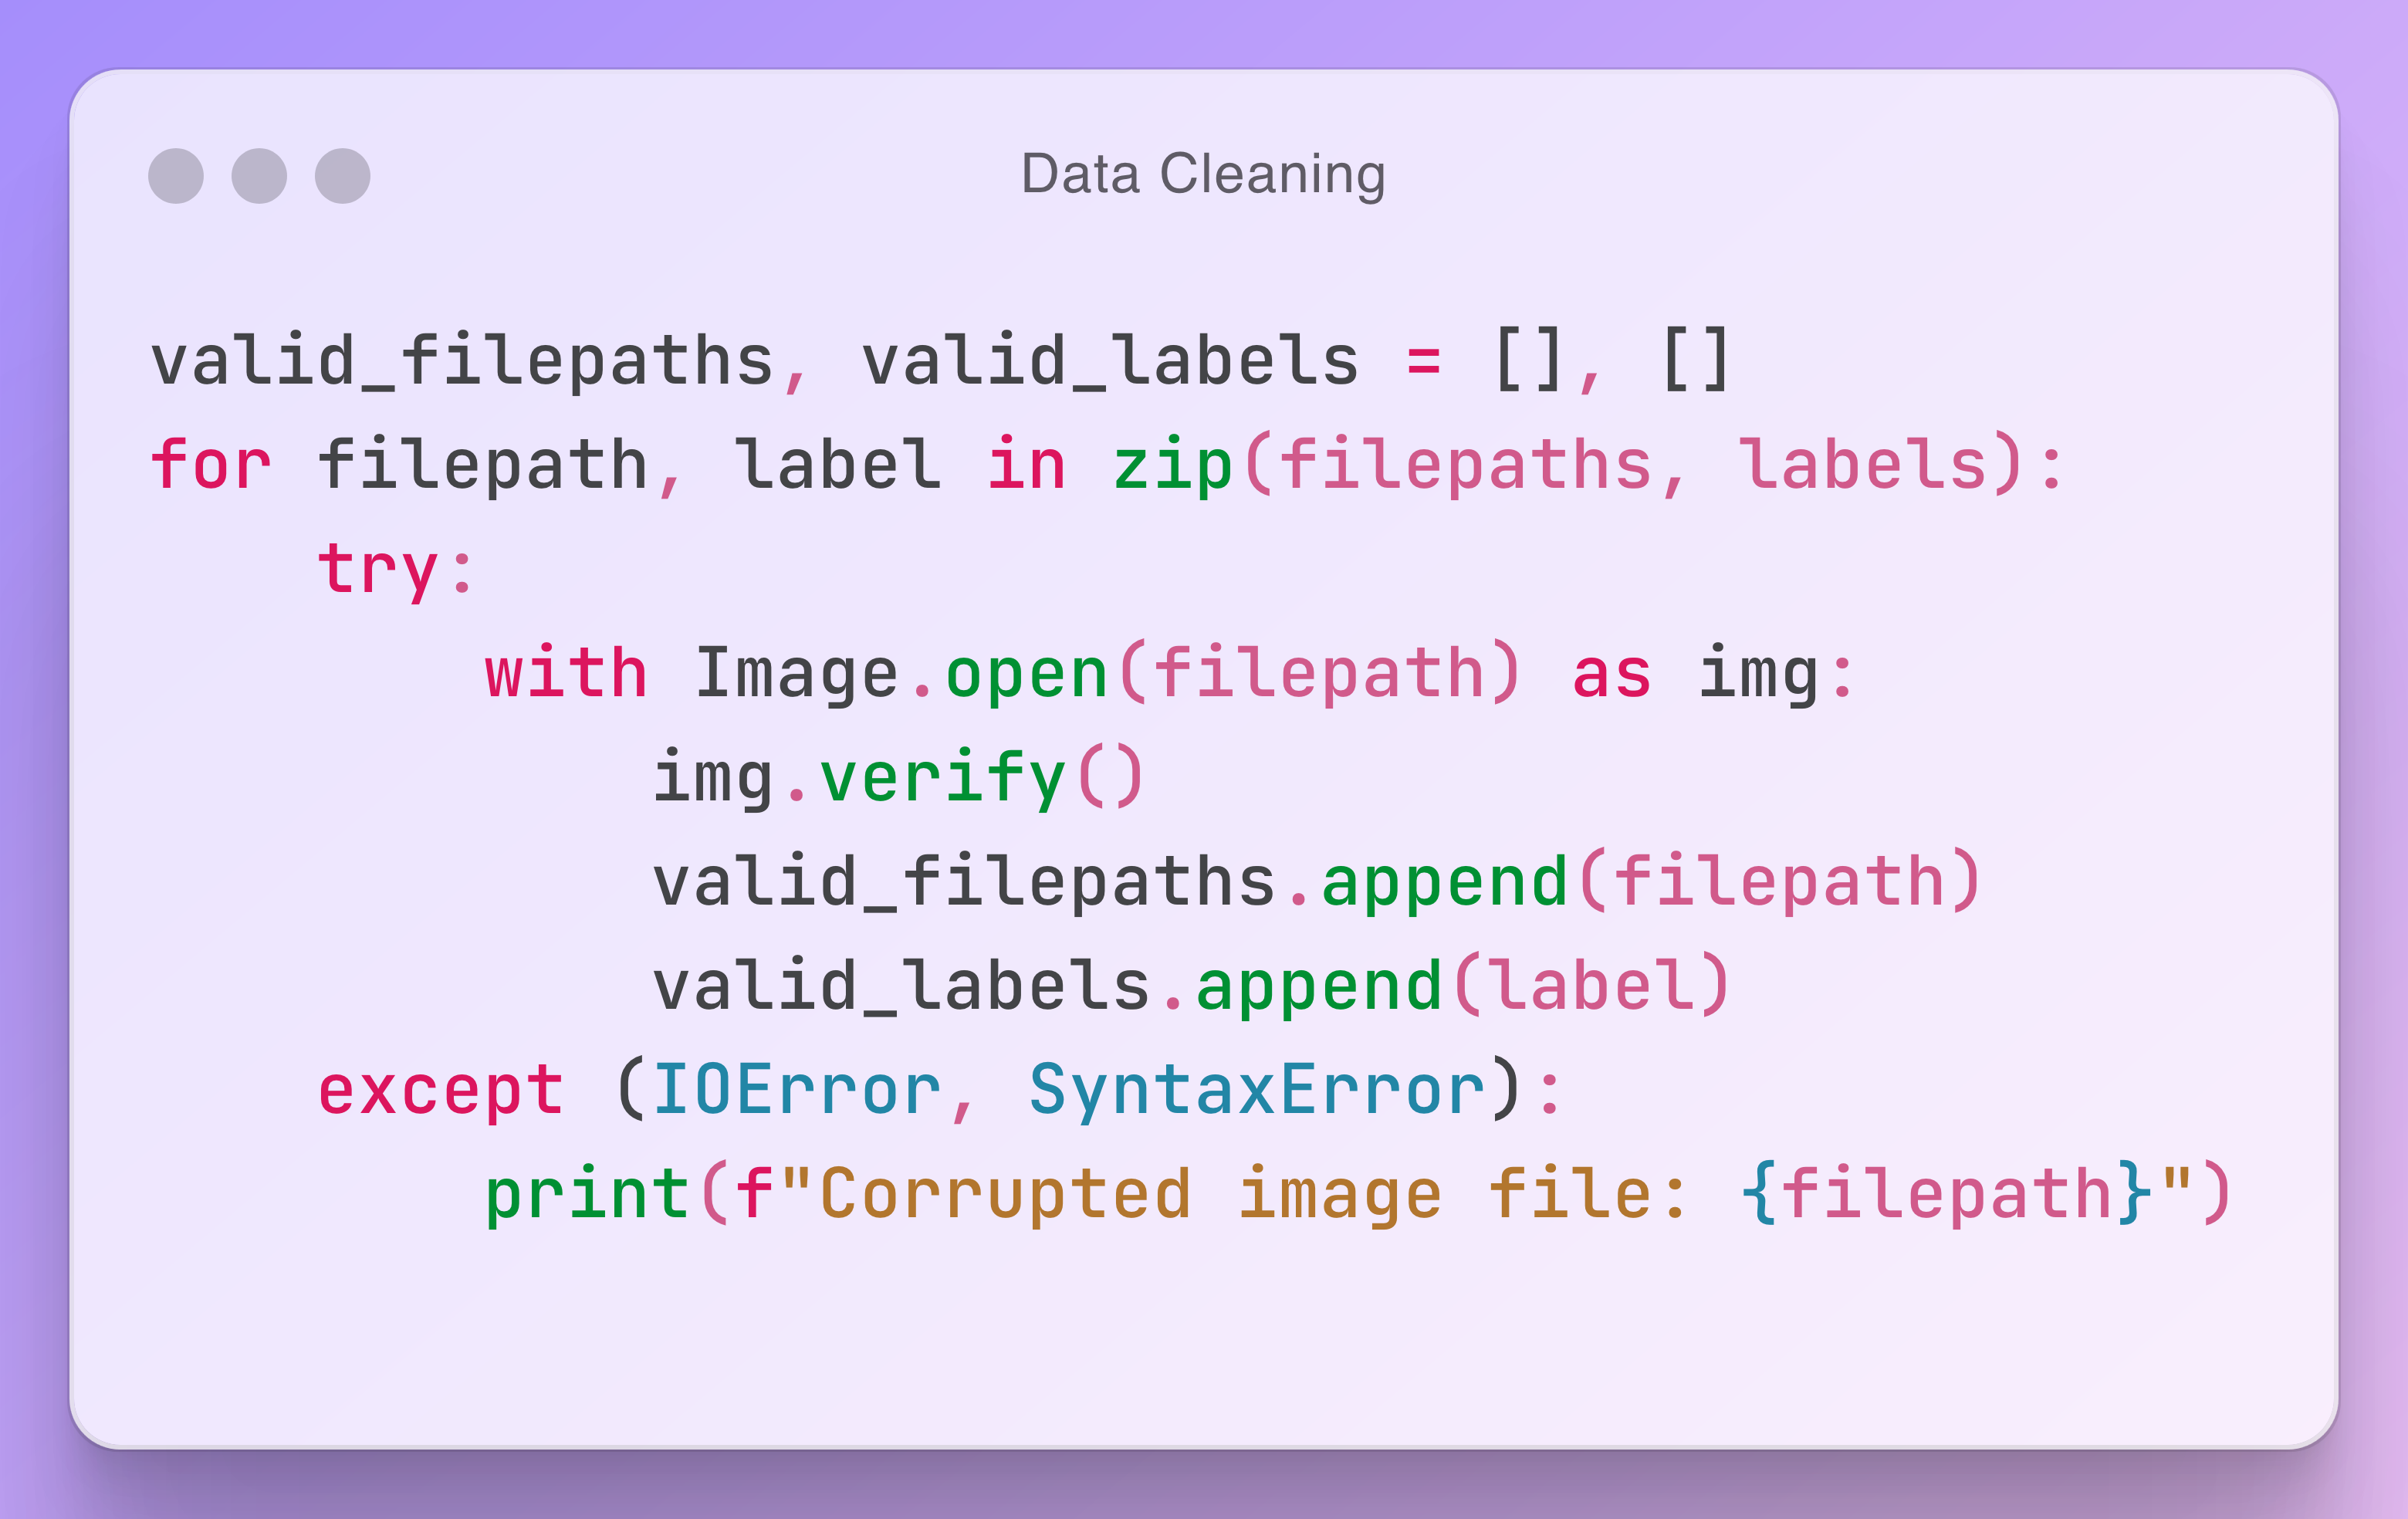
\includegraphics[width=0.8\columnwidth]{figures/data_cleaning.png}  % Adjust the width to your liking
    \caption{Dataset cleaning} % Caption for the image
    \label{fig:dataset_Cleaning} % Label to reference the image later in the document
\end{figure}
In this step the corrupt image will be removed if incase any are found. But in this particular dataset we were not getting error. Hence none of the image were deleted from the dataframe.

\subsection{Data Resizing}
The images are resized into the size of to $224 \times 224$ pixels. This is because the model that we are using i.e. EfficientNet-B0 are designed for a specific image size that is $224 \times 224$ pixels. That is because EfficientNet-B0 uses compound scaling method where the width of the network, depth and the resolution are uniformly scaled. If the input sizes are changed the performance and the efficiency of model will be hampered. And accuracy of the model will be lowered. And if higher pixels are used then there will not be any performance gains but just extra effort while training the data . Hence we have to scale it down to that size \cite{tan2019efficientnet} \cite{efficientnet_medium} \cite{keras_efficientnet}. While it is possible to input the sizes like  $244 \times 244$ the performance of the model will be degrading hence it is better to get the input size as the one that is well optimized for for the best results. 

\subsection{Color Mode}
The image color is chosen to be in RGB more. Generally, the color in all the digital images and displays is usually RGB (Red, Green, Blue). By using these three primary colors in different intensities, the model will be able to find patterns in a wider range of hues \cite{epackprinting_rgb}. RGB is considered to be a standard right now as input for many trained convolution neural networks (CNNs) \cite{dsp_rgb_hsv}. Using RGB images guarantees compatibility with these models, allowing for transfer learning and the utilization of pre-existing architectures. In many image identification tasks, color is an essential element. Because RGB photos preserve all the color information, models may recognize and learn complex patterns from color fluctuations much better than using the black-and-white color modes. This is especially beneficial for image classification tasks.

\subsection{Class Mode}
So the generator is told to give one-hot encoded labels,' where each label will have its own unique pattern in vector form \cite{loss_functions_image_classification}. Only one indices in the vector will have value other indices will be zero. That way the model will be able to understand which image is of which class. Training models with categorical is a common loss function in the case of multi-class classification.\cite{generalization_cross_entropy} The categorical cross-entropy loss function, commonly used in multi-class classification, goes well with one-hot encoded labels. This loss function efficiently calculates the difference between the actual distribution and the predicted probability distribution. Hence, by utilizing category labels, the model can generate a probability distribution for all categories \cite{robust_multiclass_classification}.

\subsection{Batch size}
In the preprocessing step a batch size of 32 is chosen for training. This will ensure that there is a balance between computational efficiency and model performance. Smaller batch sizes like 32 offer a trade-off between efficiency and gradient stability, potentially helping escape local minima and generalize better. They fit within modern GPUs’ memory constraints while maintaining stability \cite{keskar2017largebatchtrainingdeeplearning}. Larger batch sizes will be even though smoother it will require require alot more more memory and there is a high risk of overfitting.Additionally, batch size affects convergence speed, allowing sufficient weight updates without excessive overhead, balancing training speed and learned representation quality \cite{masters2018revisitingsmallbatchtraining}.

\subsection{Normalization}
The images are preprocessed using\texttt{preprocess\_input} normalization for the model, this is by using the  function from the EfficientNet library itself. This was used so that input images are properly scaled as required by the model itself. This ensures that the images are standardized by transforming pixel values into a range that aligns with the data the model was trained on. This kind of normalization becomes very much important in deep learning models to that it can improve the performance and efficiency of the models\cite{tan2019efficientnet}.

The approach used in EfficientNet's \texttt{preprocess\_input} function will rescale values of the pixelfrom their original range of $[0, 255]$ to $[-1, 1]$. In this process it subtracts the mean and divided it by the standard deviation of pixel values.The formula for normalization is:

\[
\text{Normalized Pixel Value} = \frac{\text{Pixel Value} - \mu}{\sigma}
\]

where:
\begin{itemize}
    \item $\mu$ represents the mean of the pixel values across the dataset.
    \item $\sigma$ stands for the standard deviation of the values of the pixel values across the dataset.
\end{itemize}

Normalizing the image will ensures that all input data will lie withing a similar scale this will prevent the issues issues like convergence caused due to having large variations in input magnitudes \cite{he2015delving}.

\section{Proposed Model Architecture}
This section outlines the about the model architecture that is used for this research. The model of choice for this task is EfficientNetB0. It is a very powerful and efficient pertained model that extracts the features and then will be used to include uncertainty estimation into the pipeline. This will help in improving the reliability in these models for the clinical environment.

\subsection{Base Model Architecture}
\begin{figure}[h!]
    \centering
    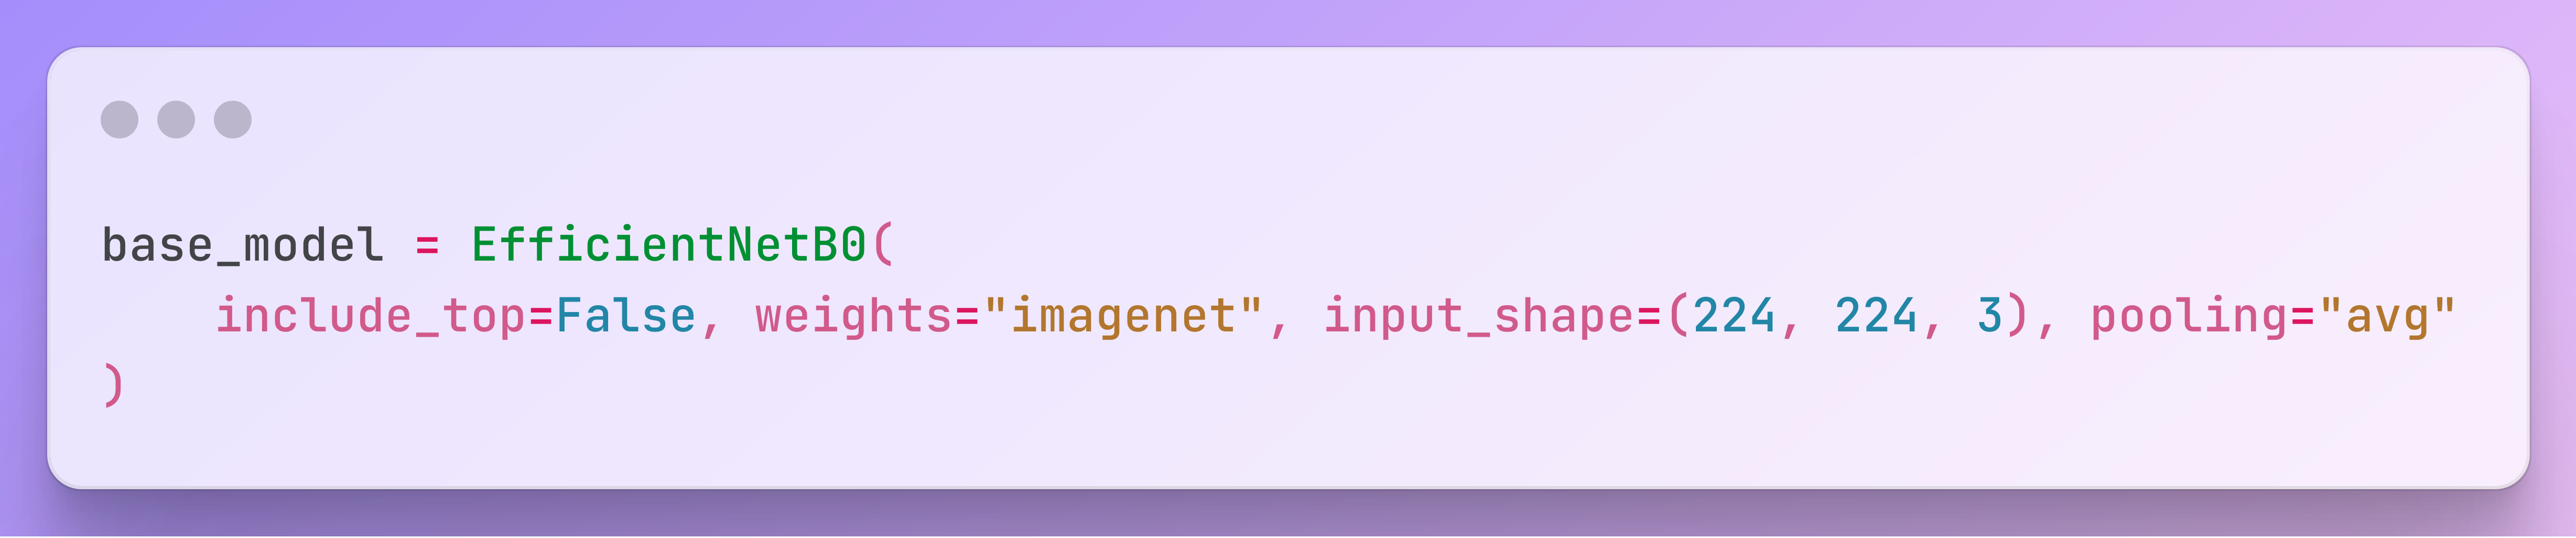
\includegraphics[width=0.8\columnwidth]{figures/model_base.png}  % Adjust the width to your liking
    \caption{Model Base} % Caption for the image
    \label{fig:base model} % Label to reference the image later in the document
\end{figure}
EfficientNet is considered to be one among the best models in the world on Convolution Neural Network. It is known to be one of the best models made for these sort of tasks which is able to do it much more efficiently but not compromising the performance. EfficientNetB0 known for its efficient scaling of depth, width, and resolution and it is used as backbone of the proposed model \cite{2021Hoang}. The network will be initialized with pre-trained ImageNet weights so as to make use of the transfer learning. The architecture includes global average pooling at the output of the backbone, followed by a fully connected layer with 128 neurons and a ReLU activation function. A Dropout layer with a rate of 0.3 is introduced to prevent overfitting. And the input shape of the images will be set to $224 \times 224$ pixels as expected by the EfficientNetB0 model for best performance.

\subsection{Adding Uncertainty Estimation}
As seen in the paper that have been working on Alzheimer’s detection problem, inclusion of uncertainty/confidence parameters for the output to show the confidence of the models is something that is used little to none. Inclusion of this parameter will give the clinicians an idea of how confidently the model is been able to classify the image into that class. In this study to quantify uncertainty, Monte Carlo (MC) Dropout is been used during inference step. This means a dropout layer will be included while conducting the prediction to perform multiple stochastic forward passes. To calculate the uncertainty, we use the standard deviation of the predictions across all these passes. Let’s break down the formal definition of uncertainty for a set of $n$ forward passes:

\begin{equation}
\sigma = \sqrt{\frac{1}{n} \sum_{i=1}^{n} (p_i - \bar{p})^2},
\end{equation}
here $p_i$ stands for the prediction for the $i$-th forward pass, and $\bar{p}$ is the mean prediction.

\subsection{Output Layer}
\begin{figure}[h!]
    \centering
    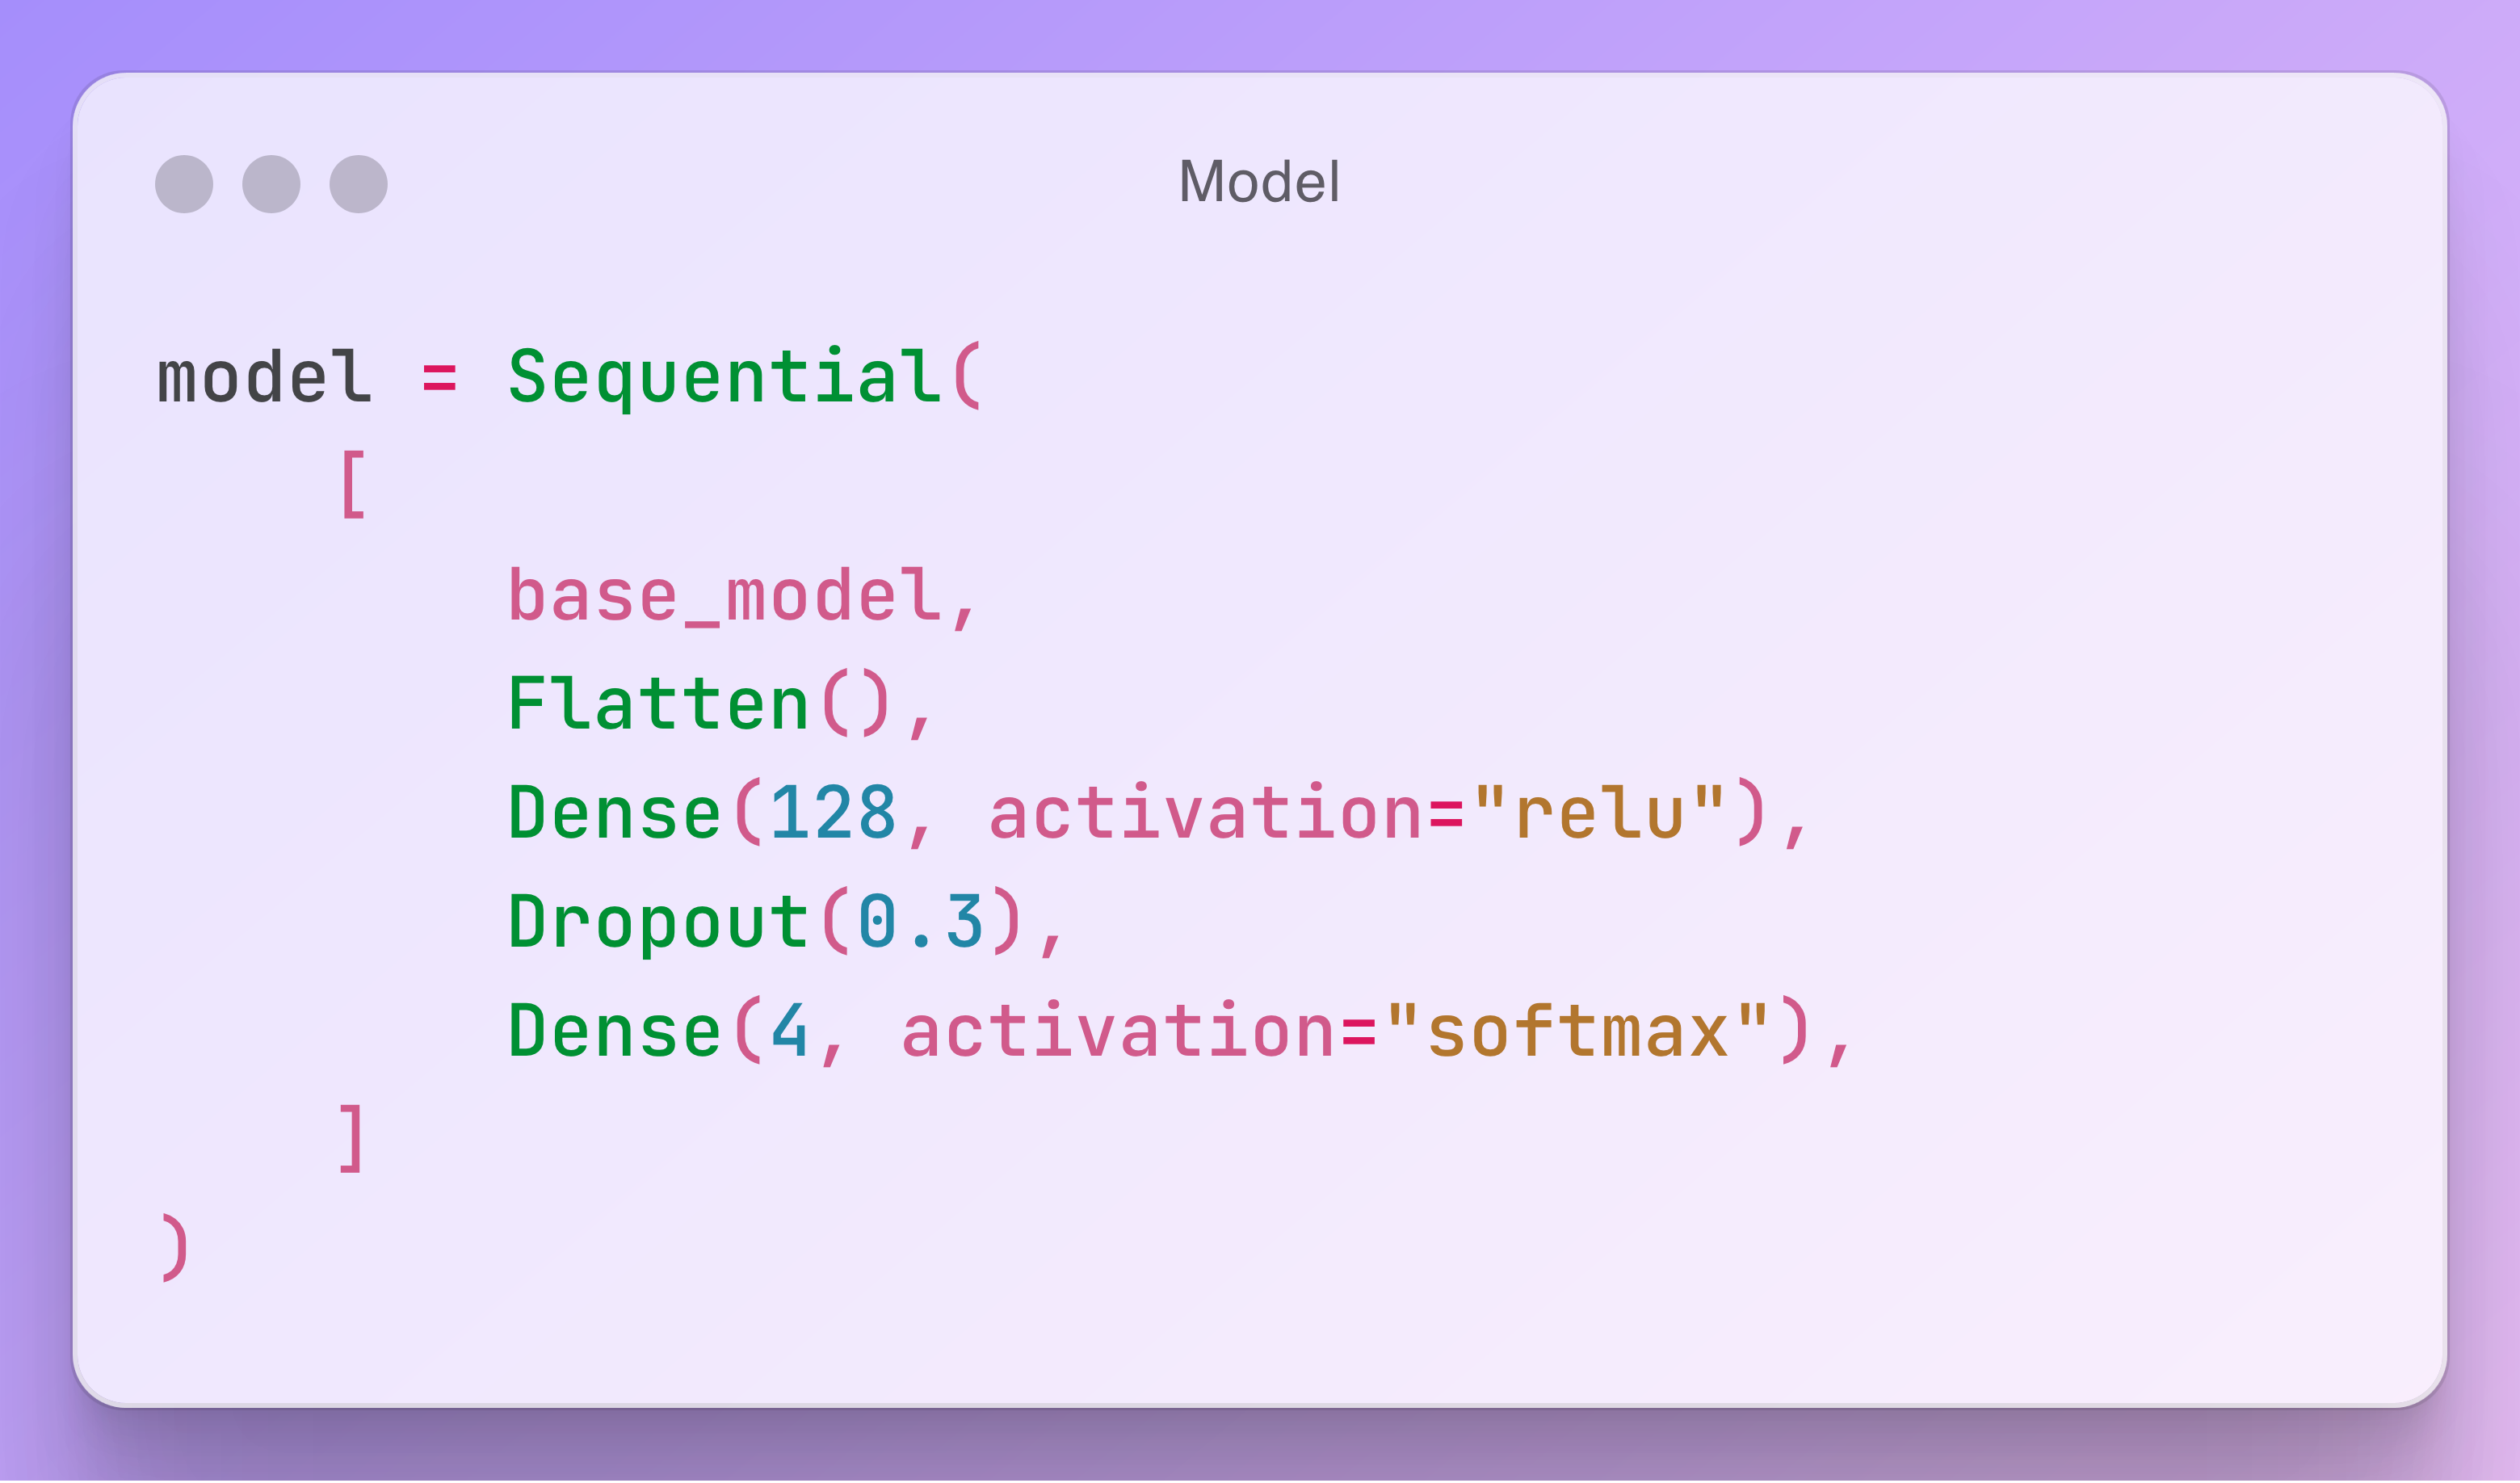
\includegraphics[width=0.8\columnwidth]{figures/model_sequential.png}  % Adjust the width to your liking
    \caption{Model sequential} % Caption for the image
    \label{fig:sequential model} % Label to reference the image later in the document
\end{figure}
The output layer has 4 neurons. This is because there are four different classes that the model will be predicting. Hence there are four neurons. The activation layer user for the final output layer is 'softmax'. The output layer will be creating probability scores for each class: NonDemented, MildDemented, VeryMildDemented and ModerateDemented. 

\subsection{Training and Evaluation}
The model is compiled using the Adamax optimizer with a learning rate of 0.001. The categorical crossentropy loss function is employed to optimize multi-class classification performance. Early stopping and learning rate reduction strategies are implemented to ensure robust convergence.

The model is trained on the training dataset for $N$ epochs with validation monitoring. Performance metrics, including accuracy, precision, recall, and F1 score, are computed on the test dataset. Monte Carlo predictions are utilized during evaluation to derive the mean prediction and uncertainty values.


\section{Model Training and Optimization}

\subsection{Training Configuration}
This step is consider to be the most critical steps in the machine learning process. How model is configured has a huge impact on the models perfomance on the final task as well as the efficiency of the model while training as well while predicting the results. The model used here make use of the Adamax optimizer. It is a variant of the Adam optimizer. But we make use of Adamax optimizer particularly because Adamax is suits extremely well for the sparse gradients and high dimensional data.So it fit's well for the image dataset that we are using. The learning rate is set to \(0.001\). In several studies it has been showed that learning rate of \(0.001\) balances convergence speed and model stability as it has been demonstrated in prior studies to balance convergence speed and model stability \cite{2017Kingma}. The categorical crossentropy loss function is utilized as this is a multi class classification. It has proved to be very effective for the multi-class classification.The Formula for categorical crossentropy is as follows \ref{eq:categorical_crossentropy}:

\begin{equation}
    L = -\sum_{i=1}^{N} y_i \log(\hat{y}_i),
    \label{eq:categorical_crossentropy}
\end{equation}
here \(y_i\) stands for the true label, and \(\hat{y}_i\) stands for the predicted probability for the \(i\)-th class.

\subsection{Optimization Strategies}
To improve the model's generalization, the proposed model introduces two optimization strategies: Early Stopping and Learning Rate reduction

\subsubsection{Early Stopping}
Introduction of the Early stopping while training model will make sure the the validation loss in always monitored. And when performance of the validation set does not improve it will stop the training, once the patience period is reached. This will ensure that the model is not overfitted for the test model. This is improve the generalizability of the model. And also this will prevent the unnecessary computation power that is required \cite{1996Lutz}. The patience parameter is set to five epochs. The parameter \texttt{restore\_best\_weights} will make sure thaat model always comes back to it's best-performing weights. This is an example algorithm \ref{alg:early_stopping} showing the same.

\begin{algorithm}[h]
\caption{Early Stopping}
\label{alg:early_stopping}
\begin{algorithmic}[1]
\State Set's patience \( p \) to 0
\For{every epoch}
    \If{Validation loss improves}
        \State Saves the model weights
        \State Resets patience \( p \) equals 0
    \Else
        \State Increments patience \( p \) by 1
    \EndIf
    \If{p is >= to patience}
        \State Training will be Stopped
    \EndIf
\EndFor
\end{algorithmic}
\end{algorithm}

\subsubsection{Learning Rate Reduction on Plateau}
If the learning rate doesn’t improve for three epochs in a row, we decrease it by half. This way, the model finds a better local minimum and keeps training stable. \cite{2017Loshchilov} says this method works really well. After the reduction, we calculate the new learning rate \(lr_t\) as follows:

\begin{equation}
    lr_t = \max(f \cdot lr_{t-1}, lr_{\text{min}}),
\end{equation}
where \(f\) is the reduction factor, \(lr_{t-1}\) is the learning rate in the previous epoch, and \(lr_{\text{min}}\) is the minimum allowable learning rate.

\subsection{Training Process}
The model training process was done using 10 epochs, on the training set and then it is validated on the validation set. So that model can be evaluated on each epoch. The history which training will be saved which included parameters such as accuracy, loss information. These evaluation are being saved for both the sets i.e. training set as well as the validation set.Table \ref{tab:training_parameters} give a overall summary of the full training process.

\begin{table}[h]
    \centering
    \caption{Training Parameters and Configuration}
    \label{tab:training_parameters}
    \begin{tabular}{|l|l|}
        \hline
        \textbf{Parameter} & \textbf{Value} \\
        \hline
        Optimizer          & Adamax \\
        Learning Rate      & 0.001 \\
        Loss Function      & Categorical Crossentropy \\
        Early Stopping Patience & 5 epochs \\
        Learning Rate Reduction Factor & 0.5 \\
        Minimum Learning Rate & \(1 \times 10^{-6}\) \\
        Epochs             & Set to 10 but it is Dynamic (Based on Early Stopping) \\
        \hline
    \end{tabular}
\end{table}

\section{Evaluation Metrics}

To evaluate the performance of the base as well as the proposed model, we will be taking into account several metrics. They are  accuracy, precision, recall, F1-score, macro average and weighted average. This will allows to get a very detailed understand of the models performance. Additionally because this is a multi class classification this thesis put light to the evaluation metrics on each classes to that it records how well it performs for each class. These metrics will provide a detailed view of how well the model is being able to make predictions for each class. Furthermore, uncertainty evaluation is being implemented in this thesis. This is something that was not included in the base model. Tell me give us idea about how confident the model is when it comes to predicting the values.

\subsection{Accuracy}
Accuracy is a very important metric while evaluating classification models, in this case a multi class classification model. Accuracy shows the ratio of correct predictions to the total number of predictions made. The formula used to calculate accuracy is as follows:

\begin{equation}
    \text{Accuracy} = \frac{\text{No. of correct predictions}}{\text{Total no. of predictions}} = \frac{\sum_{i} I(y_{\text{pred},i} = y_{\text{true},i})}{N},
\end{equation}
here \( y_{\text{pred},i} \) stands for the predicted label \( i \), \( y_{\text{true},i} \) stands for the true label, and \( N \) is the total number of samples.

\subsection{Precision}
Precision metrics will find a proportion of positive predictions that are that are actually positive. It is important for this thesis because the cost of false positive can be very risky. When it comes to medical diagnosis a false positive prediction can lead to unnecessary medications and treatments. And since the dataset is moderately imbalanced this evaluation metrics becomes very important. The formula for calculating Precision is as follows:
\begin{equation}
    \text{Precision} = \frac{TP}{TP + FP},
\end{equation}
where \( TP \) represents true positives and \( FP \) represents false positives.
In our case of Alzheimer’s diagnose it becomes important because minimizing false positive is very important to avoid over diagnosis.

\subsection{Recall}
Recall is also called sensitivity or true positive rate. Recall will be measuring the proportion of actual positive class that are correctly identified by the model. In the context of Alzheimer's disease detection, recall indicates the model’s ability to classify all potential Alzheimer’s patients. High recall ensures that fewer true positives are missed, which is crucial for early diagnosis. The formula to calculate Recall is:
\begin{equation}
    \text{Recall} = \frac{TP}{TP + FN},
\end{equation}
where \( TP \) represents true positives and \( FN \) represents false negatives.

In our case of Alzheimer’s classification it becomes where important to check if the model is failing to detect positive case of Alzheimer’s or in other words false positives. Because if the model is failing to tell the class which the patient is in then the disease might go unnoticed and it might worsen at the later stages of his/her life.

\subsection{F1-Score}
F1-score is calculated using all of the above scores. It is a 2 times the multiplication of Precision and Recall and devided by addition of Precision and Recall as shown in the equation. The Formula for F1 score is as follow: 
The F1-score is the harmonic mean of precision and recall, providing a balanced measure of the model's performance. It is particularly useful when dealing with class imbalance, as it considers both false positives and false negatives. The F1-score is defined as:

\begin{equation}
    \text{F1-score} = 2 \cdot \frac{\text{Precision} \cdot \text{Recall}}{\text{Precision} + \text{Recall}},
\end{equation}


\subsection{Confusion Matrix}
By using the confusion matrix we are able to visualize the performance of the model. Confusion matrix visualizes the number of correctly predicted items and incorrectly predicted items across all classes. This will enable to calculate the evaluation metrics like accuracy, recall, precision and F1-score for each class as shown the table \ref{tab:confusion_matrix}.

\begin{table}[h!]
\centering
\begin{tabular}{|c|c|c|c|c|}
\hline
\rowcolor[HTML]{EFEFEF} 
& \multicolumn{4}{c|}{\textbf{Predicted}} \\ \hline
\textbf{True} & \textbf{NonDemented} & \textbf{VeryMildDemented} & \textbf{MildDemented} & \textbf{ModerateDemented} \\ \hline
\textbf{NonDemented} & \cellcolor[HTML]{DFF0D8} TP1 & FN1 & FN2 & FN3 \\ \hline
\textbf{VeryMildDemented} & FP1 & \cellcolor[HTML]{DFF0D8} TP2 & FN3 & FN4 \\ \hline
\textbf{MildDemented} & FP2 & FP3 & \cellcolor[HTML]{DFF0D8} TP3 & FN5 \\ \hline
\textbf{ModerateDemented} & FP4 & FP5 & FP6 & \cellcolor[HTML]{DFF0D8} TP4 \\ \hline
\end{tabular}
\caption{Confusion Matrix for Model Evaluation}
\label{tab:confusion_matrix}
\end{table}

\subsection{Uncertainty Estimation}
Along with all the standard classification metrics that are used in previous researches, in this research models uncertainty while predicting the class in being calculated. For this task the chosen method is Monte Carlo Sampling. For each prediction the model will evaluate multiple times, and the variance which predicting among all samples is used to calculate uncertainty. The predicted mean and the uncertainty is calculated using the below formula:

\begin{equation}
    \text{mean predictions} = \frac{1}{N_{\text{samples}}} \sum_{i=1}^{N_{\text{samples}}} \hat{y}_i,
\end{equation}
\begin{equation}
    \text{uncertainty} = \sqrt{\frac{1}{N_{\text{samples}}} \sum_{i=1}^{N_{\text{samples}}} (\hat{y}_i - \text{mean predictions})^2},
\end{equation}
where \( \hat{y}_i \) represents the \( i \)-th prediction, and \( N_{\text{samples}} \) is the number of Monte Carlo samples \cite{2016Gal}.

In this study, we used 5 samples for each test input, and the predictions with higher uncertainty (above a threshold of 0.2) were identified to assess where the model's confidence is low.

\subsection{Performance Evaluation on Test Set}

The model's performance was evaluated on the test set using the metrics discussed above. The test accuracy was computed and reported, along with the confusion matrix, as shown in Table \ref{tab:confusion_matrix}. Additionally, class-specific metrics such as precision, recall, and F1-score were calculated and displayed in a detailed classification report.

\subsection{Model Saving and Loading}

Once the evaluation metrics were computed, the model was saved to disk for future use. The model's architecture and weights were stored in a Keras-compatible format:

\begin{quote}
    \texttt{model.save('path/to/save/model')}.
\end{quote}

The saved model was then reloaded for subsequent testing and predictions using the following code:

\begin{quote}
    \texttt{model = tf.keras.models.load\_model('path/to/load/model')}.
\end{quote}

\section{Pipeline Integration}

The final model is integrated into a Flask-based web application, enabling clinicians to upload MRI scans and visualize predictions with confidence scores.

\section{Implementation Details}

The model is developed using PyTorch and trained on an NVIDIA RTX 3090 GPU with 24 GB VRAM. A detailed workflow of the pipeline is illustrated in Figure~\ref{fig:pipeline}.

% \begin{figure}[h!]
%     \centering
%     \includegraphics[width=0.8\textwidth]{pipeline_diagram.png}
%     \caption{Proposed Pipeline Workflow}
%     \label{fig:pipeline}
% \end{figure}


\chapter{Results}
Your results go here.

\chapter{Discussion}
Your discussion goes here. 123456

\chapter{Conclusion}
Your conclusion goes here.

\chapter*{Acknowledgements}

First of all, I like to thank my Professor, Prof. Dr. Mazhar Hameed, for their invaluable guidance, encouragement, and their continuous input and support throughout this research. Their expertise in the field of machine leaning and the insights provided by them have been have been a great value add for me in this thesis journey. They have also given their valuable hours towards me to discuss with about the updates and guide me to the right direction. Even though they had a busy schedule, they mangaged to squeeze some time of for me which helped me achieve great progress in this whole thesis.

I am also very thankful to the faculty and staff of Gisma University of Applied Sciences for providing a supportive academic environment and access to the resources necessary for conducting my research. 

A sincere thank you goes to all my friends and colleagues, who offered encouragement, shared knowledge, and supported me throughout this journey. All of Their companionship and moral support have been a source of motivation during challenging times. I would like to express my deepest gratitude to my family for their unwavering love, patience, and understanding. Their belief in my abilities has been my greatest source of strength and inspiration. As special thanks to partner who has been very support to me in this entire thesis duration.

This thesis is dedicated to everyone who contributed to making this research a reality. Thank you all for your profound impact on my academic and personal growth.


\begin{flushright}
\textit{Jason Joel Pinto} \\
\textit{22 December 2024}
\end{flushright}

% Appendices
\appendix
\chapter{Appendix Title}
Appendix content goes here.

% References
\cleardoublepage
\printbibliography
\end{document}